\begin{figure}[htbp]
  \centering
  
\includegraphics[width=0.92\textwidth]{figures/ICA1_embed_1.png}
  \caption{}
  \label{fig:ica1_1}
\end{figure}

\chapter{Abstract}

The rapid adoption of Internet of Things (IoT) devices within domestic and small-to-medium business (SMB) environments has significantly expanded the digital attack surface, often without a corresponding increase in security awareness or technical capability among end users (Fortinet, 2024; Bugcrowd, 2026). Many consumer and SMB IoT deployments rely on devices that lack robust security controls, have limited visibility, and provide little or no notification when devices are compromised, taken offline, or interfered with through deliberate disruption such as Wi-Fi jamming (TechHive, 2024; Journal of Engineering 360, 2024).

This project presents the design and development of a security monitoring application that focuses on device availability, anomaly detection, and proactive alerting for IoT environments. The system is intended to operate without additional hardware, making it accessible and cost-effective for non-expert users.

The project adopts a full lifecycle approach, incorporating requirements analysis, system design, implementation, and evaluation. Core functionality includes device registration, continuous heartbeat monitoring, anomaly detection based on connectivity and behavioural indicators, and multi-channel alerting. The effectiveness of the proposed solution is evaluated through functional testing and simulated failure scenarios. The report concludes with a critical appraisal of the system's limitations and outlines potential future enhancements, including scalability improvements and advanced anomaly detection techniques.

\chapter{Introduction}

\section{Project Context}

Internet of Things (IoT) has become an integral component of modern digital infrastructure, particularly within residential and small to medium business (SMB) environments. Smart cameras, doorbells, thermostats, health devices, and industrial sensors are increasingly deployed to improve efficiency, safety, and convenience. Industry reports indicate sustained growth in the number of connected devices globally, with consumer and SMB deployments accounting for a significant proportion of this expansion (IoT Analytics, 2024).

However, this rapid adoption has not been matched by equivalent advances in user-level security awareness or protective controls. Unlike enterprise environments, which typically deploy dedicated intrusion detection systems (IDS), security information and event management (SIEM) platforms, and trained security personnel, home and SMB users often rely on default device configurations and minimal router-level protections (Hassan et al., 2020). As a result, many IoT devices operate with limited monitoring, poor visibility, and inadequate alerting mechanisms. When devices fail, are tampered with, or are deliberately disrupted, users may remain unaware for extended periods, increasing both security and safety risks.

\section{Problem Statement}

A central problem addressed by this project is that many IoT devices provide little or no meaningful feedback to users when they are compromised, disconnected, or rendered unavailable. Deliberate interference techniques such as Wi-Fi jamming or network level disruption can silently disable devices without triggering alerts, leaving users with a false sense of security (TechHive, 2024). For example, a security camera or smart alarm may appear operational while it has lost network connectivity or is no longer reporting data.

Existing consumer solutions tend to focus on individual devices rather than providing holistic monitoring across an entire IoT environment (ENISA, 2023). Conversely, enterprise grade monitoring and detection systems are typically complex, expensive, and unsuitable for non-expert users. This creates a gap between consumer convenience products and professional security solutions, particularly for SMBs that require greater assurance than typical home users but lack enterprise level resources.

The problem is therefore twofold: first, there is insufficient visibility into the real-time operational status of IoT devices in home and SMB settings; second, there is a lack of affordable and user-friendly tools capable of detecting anomalous behaviour and availability issues across heterogeneous IoT deployments.

\section{Aim and Objectives}

The primary aim of this project is to design and implement a security monitoring application that enhances visibility, availability awareness, and anomaly detection for IoT devices in home and SMB environments.

To achieve this aim, the project pursues the following objectives:

To analyse common security and availability risks affecting IoT devices in home and SMB contexts.

To define functional and non-functional requirements for a lightweight IoT monitoring platform that does not rely on additional hardware.

To design a system architecture capable of registering devices, monitoring their operational status, and detecting anomalous behaviour.

To implement a prototype application incorporating heartbeat monitoring and alerting mechanisms.

To evaluate the effectiveness of the system through structured testing and simulated failure scenarios.

To critically reflect on the limitations of the solution and identify opportunities for further development.

\section{Scope of the Project}

The scope of this project is intentionally focused on monitoring, availability detection, and anomaly awareness rather than deep packet inspection or full network intrusion prevention. The system is designed to support a range of IoT devices typically found in home and SMB environments, regardless of manufacturer, provided that basic connectivity and identification can be established.

The project does not aim to replace enterprise IDS or SIEM platforms, nor does it attempt to perform invasive traffic analysis that may raise ethical or legal concerns. Instead, it focuses on lightweight, behaviour-based indicators such as device presence, heartbeat consistency, and connectivity changes. The solution is implemented as a software-based platform, avoiding the need for specialist hardware or complex network reconfiguration.

\section{Constraints and Assumptions}

Several constraints influence the design and implementation of the project. These include limitations on development time, the requirement to produce a prototype rather than a fully commercialised system, and the need to operate within the technical skills and resources available to an undergraduate project. Additionally, the system assumes that monitored devices are connected via IP-based networks and that users consent to the monitoring of device status information.

Legal and ethical considerations also impose constraints, particularly relating to data protection and user privacy. The project therefore avoids unnecessary personal data and adheres to principles aligned with the General Data Protection Regulation (GDPR).

\section{Structure of the Report}

This report is structured as follows. Chapter 6 presents background research and further elaborates on the problem domain. Chapter 7 reviews relevant literature and existing solutions within the field of IoT security and monitoring. Chapter 8 defines the system requirements and specifications. Chapter 9 describes the system design, while Chapter 10 details the implementation process. Chapter 11 evaluates the system through testing and analysis. Chapter 12 provides a critical reflection on the project and discusses limitations and lessons learned. Chapter 13 outlines potential future developments, and Chapter 14 concludes the report.

\chapter{Background and Problem Definition}

\section{Growth of IoT and Expanding Attack Surface}

The Internet of Things (IoT) ecosystem has expanded rapidly over the past decade, with connected devices now embedded across residential and small-to-medium business (SMB) environments. Devices such as smart cameras, doorbells, alarms, lighting systems, health monitors, and industrial sensors are increasingly deployed to improve convenience, automation, and operational efficiency. While this proliferation delivers tangible benefits, it also significantly increases the attack surface available to malicious actors.

Research has consistently highlighted systemic weaknesses within consumer and SMB IoT deployments, including default credentials, infrequent patching, insecure communication protocols, and limited monitoring capabilities. Recent industry analyses reaffirm that limited hardware capacity, insecure APIs, and poor device lifecycle management continue to exacerbate these vulnerabilities in modern smart homes and SMBs (Keyfactor, 2024; RiskRecon, 2023). Furthermore, securing these environments requires a systematic approach specifically tailored to the unique resource constraints of IoT devices, moving beyond the enterprise-grade solutions that are often too heavy for consumer hardware (Hassan et al., 2020). Consequently, security incidents affecting IoT devices may go undetected for extended periods, allowing attackers to exploit devices for surveillance, lateral movement, or disruption.

\begin{figure}[htbp]
  \centering
  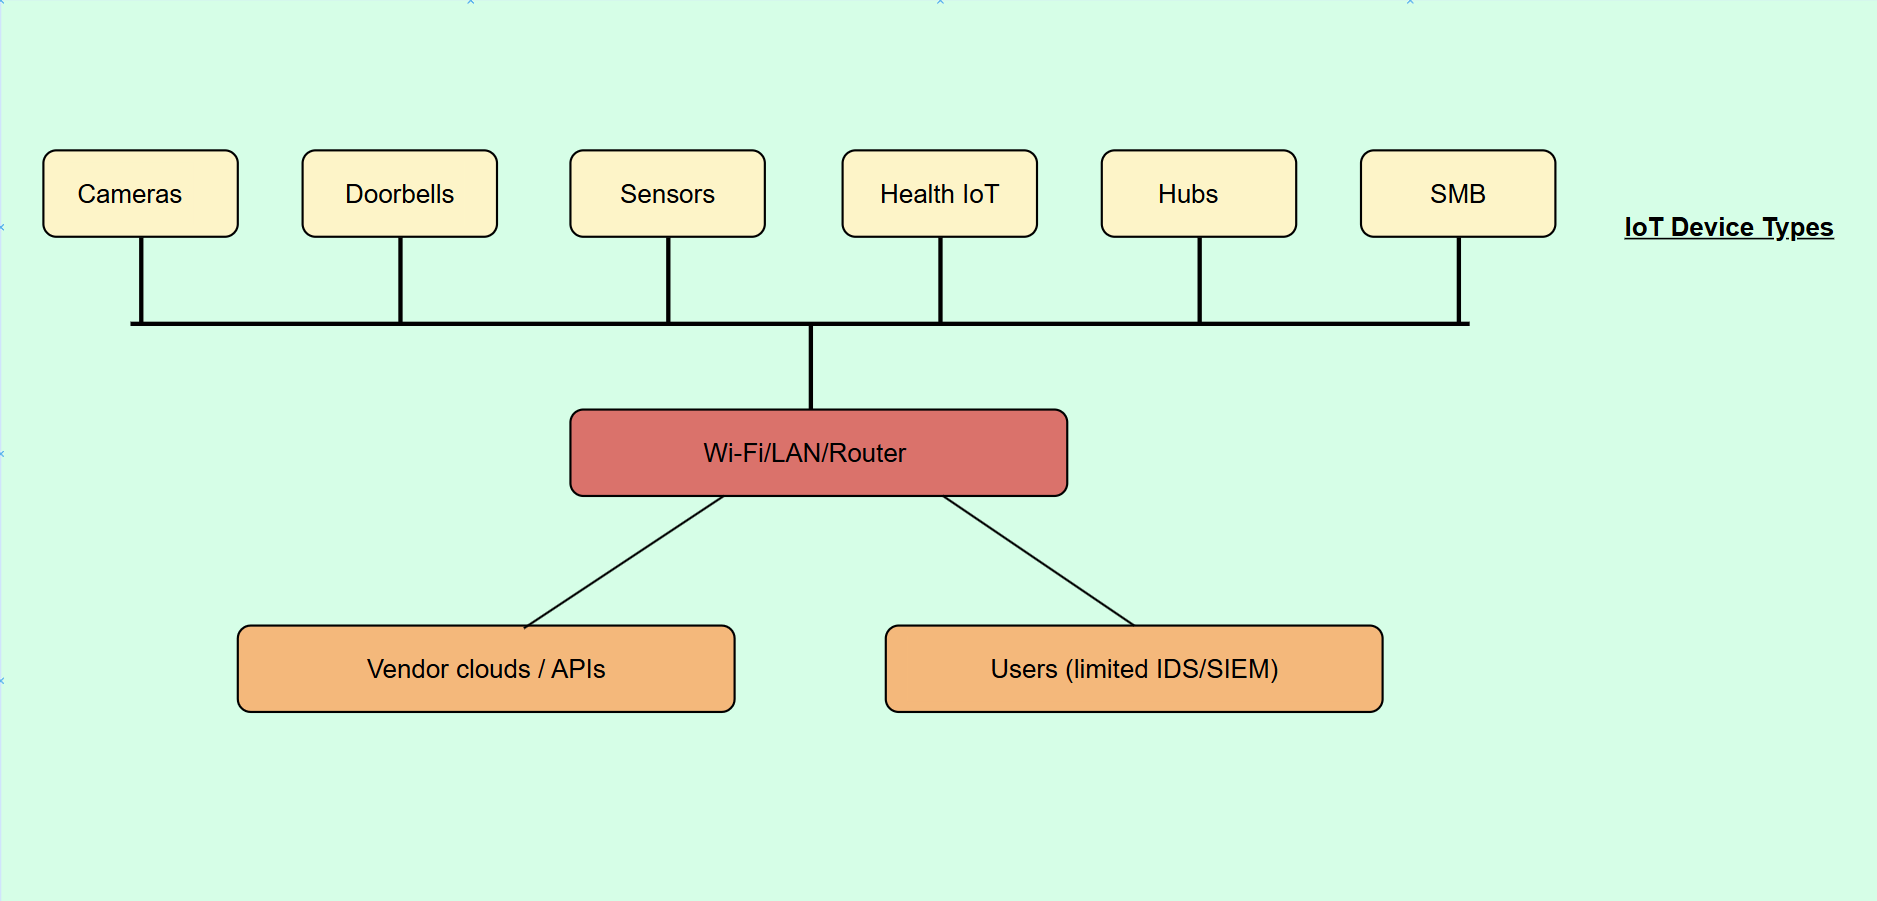
\includegraphics[width=0.92\textwidth]{figures/ICA1_embed_2.png}
  \caption{Figure  Expansion of the digital attack surface as IoT devices multiply in home and SMB environments}
  \label{fig:ica1_2}
\end{figure}

\section{IoT-Specific Security Threats}

IoT devices are subject to a range of security threats that differ in both scale and nature from those affecting traditional computing systems. High-profile incidents, such as large-scale distributed denial-of-service (DDoS) attacks leveraging compromised IoT devices, have demonstrated the potential impact of insecure deployments. These threats remain highly prevalent; compromised devices with weak authentication or unpatched firmware are continuously recruited into botnets to conceal malicious activities or execute escalating cyberattacks against wider organisational targets (Kaspersky, 2024).

Beyond overt compromise, more subtle threats also present significant risk. Attackers may deliberately interfere with device connectivity through techniques such as Wi-Fi jamming or network disruption, effectively disabling security-critical devices without triggering alerts. In IoT environments, jamming attacks specifically target the communication link by transmitting radio signals that intentionally lower the signal-to-noise ratio, disrupting the flow of information between sensors and their control gateways (OAE Publish, 2023).  Recent studies further highlight that lightweight physical-layer authentication is increasingly necessary to detect these availability-oriented attacks, such as jamming and battery-depletion, which cannot be mitigated by standard cryptographic means alone (Future Internet, 2026).

Availability is therefore intrinsically linked to security within IoT environments. From a security-driven perspective, loss of availability constitutes a security failure rather than merely a technical inconvenience

\begin{figure}[htbp]
  \centering
  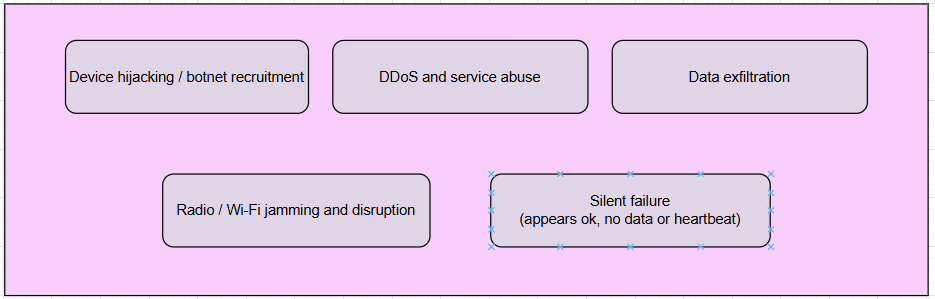
\includegraphics[width=0.92\textwidth]{figures/ICA1_embed_3.png}
  \caption{Figure  IoT-Specific threat categories relevant to availability and monitoring.}
  \label{fig:ica1_3}
\end{figure}

\section{Limitations of Existing Consumer and SMB Solutions}

Most consumer IoT products rely on proprietary vendor platforms for monitoring and alerting. While these platforms provide basic status information, they are typically limited to individual devices and lack cross-device visibility. Alerts are often restricted to application-level notifications and may fail entirely if network connectivity is disrupted. Furthermore, users are required to manage multiple applications for different device vendors, leading to fragmented visibility and poor situational awareness.

At the opposite end of the spectrum, enterprise security solutions offer comprehensive monitoring, anomaly detection, and correlation capabilities. However, these systems are expensive, complex, and require specialist knowledge to deploy and maintain. For SMBs, the cost and operational overhead of such solutions is frequently prohibitive, leaving a gap between consumer convenience products and enterprise-grade security infrastructure.

This disparity highlights a clear unmet need: a lightweight, accessible security monitoring platform that provides meaningful visibility into IoT device availability and behaviour across heterogeneous environments, without imposing enterprise-level complexity or cost.

\section{Security-Driven Availability and Anomaly Detection}

Traditional security models often treat availability as one of several security objectives, alongside confidentiality and integrity. In IoT environments, availability takes on heightened importance due to the physical and safety implications associated with device failure. Security cameras, alarms, and health monitoring devices are frequently deployed to protect people and property; their silent failure undermines trust and exposes users to risk.

Anomaly detection offers a practical approach to addressing this challenge. Rather than relying on deep packet inspection or signature-based detection, behaviour-oriented indicators such as heartbeat consistency, connectivity patterns, and device responsiveness can provide early warning of abnormal conditions. Sudden changes in device behaviour, prolonged silence, or unexpected disconnections may indicate interference, misconfiguration, or malicious activity.

A security-driven monitoring approach therefore focuses on continuous visibility and timely alerting. By identifying deviations from expected device behaviour, users can be notified promptly and take corrective action before security incidents escalate. Importantly, such an approach can be implemented without intrusive inspection of user data, reducing ethical and legal concerns.

\section{Ethical and Legal Considerations}

Monitoring IoT devices raises important ethical and legal considerations, particularly in relation to privacy and data protection. The General Data Protection Regulation (GDPR) establishes strict requirements for the collection, processing, and storage of personal data within the United Kingdom and the European Union. Any monitoring solution must therefore minimise data collection and ensure transparency regarding what information is captured and why.

This project adopts a privacy-conscious approach by focusing exclusively on device metadata and availability indicators rather than content or payload data. Monitoring is limited to information necessary to determine device status and detect anomalous behaviour, aligning with principles of data minimisation and purpose limitation. User consent is assumed as a prerequisite for deployment, and the system design avoids techniques that could be perceived as intrusive or disproportionate.

\section{Summary}

This chapter has established the background and problem context underpinning the project. The rapid growth of IoT devices within home and SMB environments has created a security landscape characterised by limited visibility, inadequate monitoring, and heightened vulnerability to both overt and subtle attacks. Existing solutions fail to adequately address these challenges, particularly with respect to availability and silent failure detection.

From a security-driven perspective, ensuring continuous awareness of device availability and behaviour is essential. The following chapter builds on this foundation by reviewing relevant literature and existing research in IoT security, monitoring, and anomaly detection, positioning the proposed solution within the wider academic and industrial context.

\chapter{Literature Review and Research Context}

\section{IoT Security Research}

Academic research has consistently identified security as a fundamental weakness within IoT ecosystems, particularly in consumer and small-to-medium business (SMB) deployments. Early work by Weber (2010) and Roman et al. (2013) highlighted the absence of unified security standards and the tension between usability, cost, and protection in IoT design. Modern literature confirms that these foundational issues persist; Hassan et al. (2020) emphasize that IoT environments still suffer from systemic vulnerabilities that demand specialized, lightweight security frameworks rather than inherited enterprise models.

A recurring theme within the literature is the disparity between enterprise security practices and those available to non-enterprise users. While large organisations typically deploy layered security controls, including intrusion detection systems (IDS), network monitoring, and continuous logging, home and SMB users rely primarily on device-level safeguards provided by manufacturers. These safeguards are often opaque, limited in scope, and insufficient for detecting sophisticated or non-traditional attacks.

Recent research has emphasised the growing importance of availability as a security property within IoT systems. Availability failures in IoT environments can have direct physical and safety implications, particularly when devices are relied upon for security monitoring or health-related functions (Sicari et al., 2015; Keyfactor, 2024). This perspective aligns with the security-driven framing adopted by this project, where loss of device availability is treated as a security incident rather than a benign fault.

\section{Intrusion Detection and Monitoring in IoT Environments}

Traditional intrusion detection systems were designed for conventional IT networks and often rely on deep packet inspection, signature-based detection, or extensive traffic analysis. While effective in enterprise contexts, these approaches are frequently unsuitable for IoT environments due to device heterogeneity, encrypted traffic, and limited processing capabilities (Zarpelão et al., 2017).

Research into IoT-specific IDS has explored lightweight and distributed detection mechanisms that minimise overhead while providing meaningful security insights. Behaviour-based monitoring has emerged as a promising alternative to signature-based techniques, focusing on deviations from normal operational patterns rather than known attack signatures. Such approaches are particularly relevant in environments where attacks may not generate obvious malicious payloads but instead manifest as changes in connectivity or responsiveness.

Several older studies proposed network-based monitoring solutions that analyse traffic flows at gateways or routers to infer device behaviour. However, more recent research has shifted toward lightweight, on-device anomaly detection and federated learning models to accommodate resource-constrained environments while preserving user privacy (Ahmad \& Shah, 2024; COMPSAC, 2025). By analysing system call arguments or utilising EdgeML, modern frameworks can achieve high accuracy in detecting resource-constraint attacks and abnormal execution phases without relying heavily on traditional network gateway bottlenecks or deep packet inspection (ResearchGate, 2025). This reinforces the need for software-centric monitoring approaches that can operate without invasive network reconfiguration.

\section{Availability Monitoring and Heartbeat Mechanisms}

Heartbeat monitoring is a well-established technique in distributed systems, used to assess the liveness and availability of nodes by verifying periodic communication signals. In the context of IoT, heartbeat mechanisms offer a lightweight and scalable method for detecting device failures, disconnections, or interference. Rather than analysing content, the system evaluates whether expected signals are received within defined time thresholds.

Research has demonstrated that heartbeat-based monitoring can be effective for identifying both accidental failures and deliberate disruption (ResearchGate, 2025). For example, prolonged absence of heartbeat messages may indicate power loss, network misconfiguration, or active interference such as jamming. Importantly, heartbeat monitoring does not require access to payload data, making it suitable for privacy-sensitive deployments (R Discovery, 2025).

Despite these advantages, heartbeat mechanisms are not without limitations. Network congestion, intermittent connectivity, or energy-saving device behaviours may result in false positives if not carefully calibrated. The literature therefore emphasises the importance of adaptive thresholds and contextual awareness when implementing availability monitoring in IoT environments to mitigate environmental noise and changing sensor behaviors without compromising privacy (R Discovery, 2025).

\section{Anomaly Detection Approaches}

Anomaly detection aims to identify deviations from expected behaviour that may indicate faults or malicious activity. In IoT contexts, anomaly detection techniques range from simple rule-based systems to advanced machine learning models. While machine learning approaches have shown promise, they often require large datasets, extensive training, and centralized computational resources that may be impractical and face scalability challenges in lightweight deployments (R Discovery, 2025).

Rule-based and heuristic-driven anomaly detection offers a pragmatic alternative for early-stage or resource-constrained systems. By defining expected behavioural patterns, such as regular heartbeat intervals or stable connectivity profiles, the system can flag anomalies when deviations occur. Recent frameworks emphasise that combining simple behavioral indicators---such as device uptime, signal consistency, and connectivity changes---can yield highly accurate anomaly detection in real-time IoT networks without the overhead of deep learning (COMPSAC, 2025; ResearchGate, 2025).

This multi-factor perspective informs the design of the proposed monitoring platform, which integrates availability and behavioural indicators rather than relying on a single metric.

\section{Commercial and Academic Solutions}

Commercial IoT security solutions typically target either individual consumer devices or large enterprise environments. Consumer-focused products often prioritise ease of use and visual feedback but provide limited diagnostic depth or cross-device correlation. Enterprise platforms, by contrast, offer comprehensive monitoring and analytics but require significant financial and technical investment that makes them difficult to govern at a smaller scale (SumatoSoft, 2025).

Academic research frequently proposes innovative detection techniques; however, many prototypes remain confined to laboratory environments and are not translated into practical tools for end users. This gap between academic research and deployable solutions is particularly evident within the home and SMB sectors, where usability and cost constraints are paramount (SecuringSam, 2023).

The proposed project seeks to bridge this gap by drawing on established research principles while delivering a practical, software-based monitoring solution tailored to non-expert users. By focusing on availability, heartbeat monitoring, and anomaly detection, the system occupies a middle ground between simplistic consumer applications and complex enterprise security platforms.

\section{Identified Research Gap}

The literature review reveals a clear research and practice gap within the IoT security landscape. While availability is widely recognised as a core security property, it is often underemphasised in consumer and SMB monitoring solutions. Existing approaches either lack holistic visibility, require specialised infrastructure, or impose unacceptable complexity on end users.

There is limited research addressing lightweight, privacy-conscious monitoring platforms that provide meaningful availability and anomaly detection across heterogeneous IoT environments without additional hardware. This project addresses this gap by proposing and implementing a security-driven monitoring application that enhances visibility, improves situational awareness, and supports timely user intervention.

\begin{table}[htbp]
  \centering
  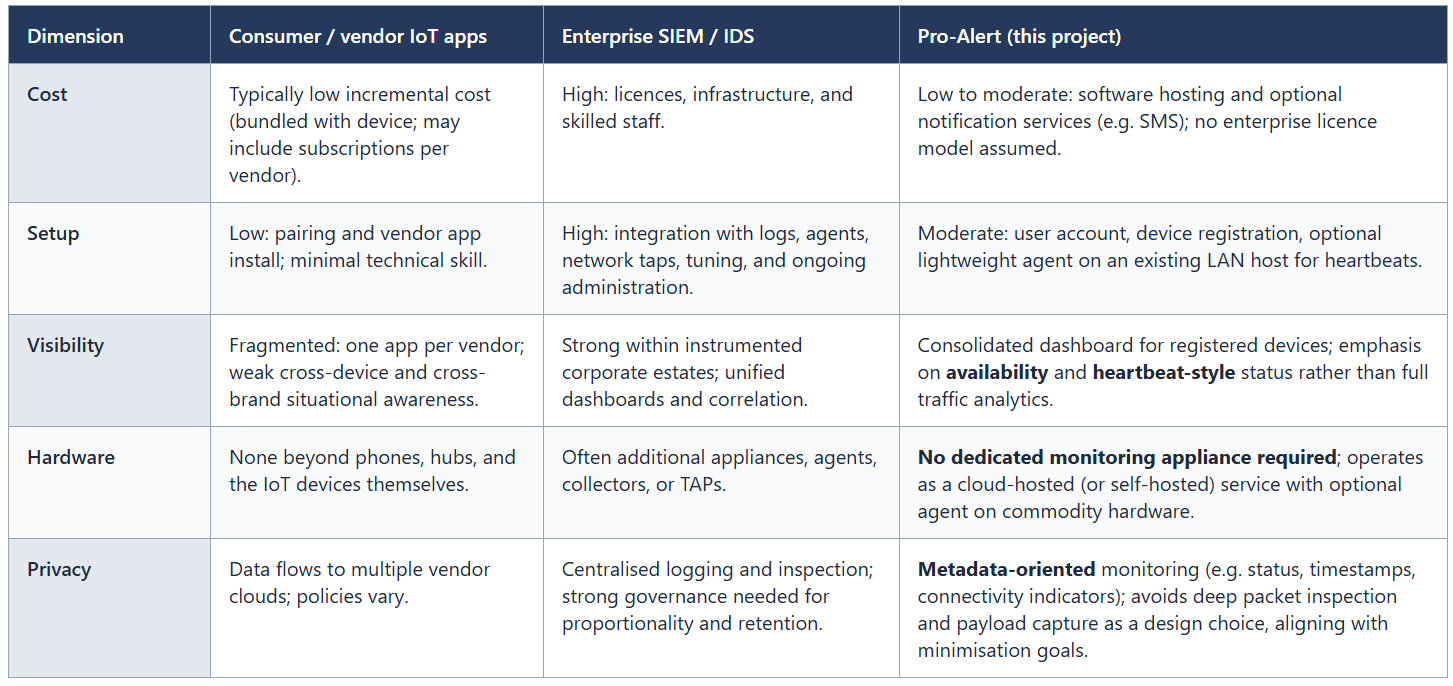
\includegraphics[width=0.92\textwidth]{figures/ICA1_embed_4.png}
  \caption{Table  Comparison of consumer IoT applications, enterprise SIEM-style monitoring, and the proposed solution across deployment and privacy dimensions.}
  \label{tab:ica1_1}
\end{table}

\section{Summary}

This chapter has reviewed relevant academic literature and existing approaches related to IoT security, monitoring, availability, and anomaly detection. The findings highlight persistent weaknesses in consumer and SMB IoT deployments and underscore the importance of availability as a security concern. The identified research gap provides a clear justification for the proposed solution.

\chapter{Requirements Analysis and System Specification}

\section{Introduction}

This chapter translates the problem context and research findings established in previous chapters into a structured set of system requirements. The purpose of the requirements analysis is to clearly define what the proposed IoT security monitoring application must achieve to meet its stated objectives. By distinguishing between functional and non-functional requirements, the project ensures that both system behaviour and quality attributes are explicitly addressed.

The requirements presented in this chapter are derived from three primary sources: the security-driven problem definition outlined in Chapter 6, the academic and industry research reviewed in Chapter 7, and practical constraints associated with home and small-to-medium business (SMB) environments. Together, these requirements form the foundation for the system design and implementation described in subsequent chapters.

\section{Stakeholders and User Roles}

The primary stakeholders for the system include home users and SMB operators who deploy IoT devices for security, automation, or monitoring purposes. These users are typically non-experts in cybersecurity and require a solution that provides meaningful insight without excessive complexity (NCSC, 2023). Secondary stakeholders include developers and system administrators responsible for maintaining the platform.

User interaction with the system is centred on a single primary role: the registered user who owns and manages IoT devices. This role is responsible for registering devices, configuring monitoring parameters, and responding to alerts. The system design deliberately avoids role complexity to maintain usability and accessibility.

\section{Functional Requirements}

Functional requirements define the specific behaviours and capabilities the system must provide. Each requirement is labelled for clarity and traceability and is directly aligned with the project objectives.

\begin{table}[htbp]
  \centering
  \small
  \caption{Table  Functional Requirements}
  \label{tab:ica1_2}
\begin{tabular}{p{0.307\textwidth}p{0.307\textwidth}p{0.307\textwidth}}
\toprule
Functional Requirement \# & Functional Requirement & Description \\
\midrule
FR1 & User Registration and Authentication & The system shall allow users to create an account and authenticate securely in order to access the monitoring platform. Authentication mechanisms must ensure that only authorised users can view device status and alerts. \\
FR2 & IoT Device Registration & The system shall allow users to register IoT devices by providing identifying information such as device name, type, and network association. Registered devices shall be uniquely identifiable within the system. \\
FR3 & Device Heartbeat Monitoring & The system shall monitor registered IoT devices through a heartbeat mechanism that verifies periodic communication or status updates. The absence of expected heartbeat signals shall be recorded as a potential availability issue. \\
FR4 & Availability Status Tracking & The system shall maintain real-time visibility of each device's availability status, including online, offline, or degraded states. Status changes shall be logged for analysis and review. \\
FR5 & Anomaly Detection & The system shall analyse device behaviour to detect anomalies, such as unexpected disconnections, irregular heartbeat intervals, or sudden changes in connectivity patterns. Detected anomalies shall be flagged for user attention. \\
FR6 & Alert Generation and Notification & The system shall generate alerts when availability failures or anomalous behaviour are detected. Alerts shall be delivered through the application interface and, where possible, through additional notification channels. \\
FR7 & Historical Data Logging & The system shall store historical device status and event data to support retrospective analysis, troubleshooting, and evaluation of device reliability. \\
FR8 & Dashboard Visualisation & The system shall provide a user-facing dashboard that presents device status, alerts, and historical trends in a clear and accessible manner. \\
\bottomrule
\end{tabular}
\end{table}

\section{Non-Functional Requirements}

Non-functional requirements define the quality attributes and constraints under which the system must operate. These requirements are critical to ensuring the system is usable, secure, and appropriate for its intended context.

\begin{table}[htbp]
  \centering
  \small
  \caption{Table  Non-Functional Requirements}
  \label{tab:ica1_3}
\begin{tabular}{p{0.307\textwidth}p{0.307\textwidth}p{0.307\textwidth}}
\toprule
Non-Functional Requirement \# & Non-Functional Requirement & Description \\
\midrule
NFR1 & Security & The system shall protect user accounts and device information through appropriate security controls, including secure authentication and access restrictions. Sensitive data shall be protected against unauthorised access. \\
NFR2 & Privacy and Data Protection & The system shall adhere to data minimisation principles and avoid the collection of unnecessary personal or payload data. Monitoring shall be limited to metadata required for availability and anomaly detection, in alignment with GDPR principles (ICO, 2024). \\
NFR3 & Usability & The system shall be intuitive and accessible to non-expert users, with minimal configuration required to achieve effective monitoring. \\
NFR4 & Scalability & The system shall support an increasing number of registered devices without significant degradation in performance, enabling use across both home and SMB environments. \\
NFR5 & Reliability & The system shall operate reliably under normal network conditions and tolerate transient connectivity issues without generating excessive false alerts. \\
NFR6 & Performance & The system shall process heartbeat signals and status updates within reasonable timeframes to ensure timely detection and alerting of availability issues. \\
NFR7 & Maintainability & The system shall be designed in a modular manner to support future enhancements, bug fixes, and feature expansion. \\
\bottomrule
\end{tabular}
\end{table}

\section{System Constraints and Assumptions}

The system is subject to several constraints that influence design and implementation decisions. As an undergraduate project, development time and resources are limited, necessitating prioritisation of core functionality over advanced features. The system is implemented as a software-based platform and does not rely on additional hardware, which constrains the types of monitoring techniques that can be employed.

It is assumed that monitored devices are connected via IP-based networks and are capable of periodic communication with the monitoring platform, either directly or indirectly. The system also assumes that users have provided informed consent for device monitoring and alerting.

\section{Requirements Traceability}

To ensure coherence between objectives, requirements, and implementation, each functional and non-functional requirement is traceable to the project aims defined in Chapter 5. This traceability supports systematic design and evaluation, demonstrating that the implemented system directly addresses the identified problem.

The following tables provide forward traceability from the project objectives in \S{}5.3 through the functional requirements (FR1--FR8) and non-functional requirements (NFR1--NFR7) defined in this chapter, to the system design (Chapter~9), implementation (Chapter~10), and testing and evaluation (Chapter~11).

\begin{table}[htbp]
  \centering
  \small
  \caption{Table  Mapping of project objectives (\S{}5.3) to report chapters.}
  \label{tab:ica1_4}
\begin{tabular}{p{0.307\textwidth}p{0.307\textwidth}p{0.307\textwidth}}
\toprule
Obj. & Objective (from \S{}5.3) & Primary evidence in report \\
\midrule
O1 & Analyse security and availability risks in home/SMB IoT & Ch.6 (background); Ch.7 (literature; including Table~1 / \S{}7.6 research gap) \\
O2 & Define functional and non-functional requirements & Ch.8 (this chapter; \S{}8.3--\S{}8.4); Tables~3--4 \\
O3 & Design architecture for registration, monitoring, anomaly detection & Ch.9 (system design) \\
O4 & Implement prototype (heartbeat, alerting) & Ch.10 (implementation) \\
O5 & Evaluate via structured testing and scenarios & Ch.11 (testing and evaluation) \\
O6 & Critically reflect; identify further development & Ch.12 (reflection); Ch.13 (future work) \\
\bottomrule
\end{tabular}
\end{table}

\begin{table}[htbp]
  \centering
  \small
  \caption{Table  FR1--FR8 mapped to design (Ch.9), implementation (Ch.10), and testing (Ch.11) subsections}
  \label{tab:ica1_5}
\begin{tabular}{p{0.153\textwidth}p{0.153\textwidth}p{0.153\textwidth}p{0.153\textwidth}p{0.153\textwidth}p{0.153\textwidth}}
\toprule
ID & Requirement (summary) & Obj. & Design (Ch.9) & Implementation (Ch.10) & Testing (Ch.11) \\
\midrule
FR1 & User registration and authentication & O2--O5 & \S{}9.3--\S{}9.4 & \S{}10.3, \S{}10.9 & \S{}11.5 \\
FR2 & IoT device registration & O2--O5 & \S{}9.4, \S{}9.8 & \S{}10.5 & \S{}11.3.1 \\
FR3 & Device heartbeat monitoring & O2--O5 & \S{}9.5 & \S{}10.6 & \S{}11.3.2 \\
FR4 & Availability status (online/offline/degraded) & O2--O5 & \S{}9.3--\S{}9.5 & \S{}10.5--\S{}10.6 & \S{}11.3.2 \\
FR5 & Anomaly detection (behaviour / connectivity) & O2--O5 & \S{}9.6 & \S{}10.7 & \S{}11.3.3 \\
FR6 & Alert generation and multi-channel notification & O2--O5 & \S{}9.7 & \S{}10.8 & \S{}11.4 \\
FR7 & Historical logging and retention & O2--O5 & \S{}9.8 & \S{}10.4, \S{}10.10 & \S{}11.3, \S{}11.6 \\
FR8 & Dashboard visualisation & O2--O5 & \S{}9.3 & \S{}10.2--\S{}10.3 & \S{}11.3 \\
\bottomrule
\end{tabular}
\end{table}

\begin{table}[htbp]
  \centering
  \small
  \caption{Table  NFR1--NFR7 mapped subsections.}
  \label{tab:ica1_6}
\begin{tabular}{p{0.153\textwidth}p{0.153\textwidth}p{0.153\textwidth}p{0.153\textwidth}p{0.153\textwidth}p{0.153\textwidth}}
\toprule
ID & Requirement (summary) & Obj. & Design (Ch.9) & Implementation (Ch.10) & Testing (Ch.11) \\
\midrule
NFR1 & Security (authentication, transport hardening, abuse resistance) & O2--O5 & \S{}9.4, \S{}9.9 & \S{}10.9 & \S{}11.5 \\
NFR2 & Privacy / data minimisation (GDPR-aligned) & O2--O5 & \S{}6.5; \S{}9.4, \S{}9.8 & \S{}10.4--\S{}10.5, \S{}10.9 & \S{}11.5 \\
NFR3 & Usability for non-experts & O2--O5 & \S{}9.3 & \S{}10.2--\S{}10.3 & \S{}11.6 \\
NFR4 & Scalability & O2--O5 & \S{}9.2, \S{}9.8 & \S{}10.10 & \S{}11.6 \\
NFR5 & Reliability / false-positive control & O2--O5 & \S{}9.5--\S{}9.6 & \S{}10.6--\S{}10.7 & \S{}11.3.2--\S{}11.3.3 \\
NFR6 & Performance (timely heartbeats and alerts) & O2--O5 & \S{}9.2 & \S{}10.10 & \S{}11.6 \\
NFR7 & Maintainability / modularity & O2--O5 & \S{}9.2, \S{}9.9 & \S{}10.3 & \S{}11.9 \\
\bottomrule
\end{tabular}
\end{table}

NFR2:~\S{}6.5 (Background --- ethical and legal context) is cited alongside Ch.9.~\S{}11.3~in FR7 refers to the functional testing block as a whole (\S{}11.3.1--\S{}11.3.3).

\section{Summary}

This chapter has defined the functional and non-functional requirements for the proposed IoT security monitoring application. By formalising system behaviour and quality attributes, the requirements analysis establishes a clear foundation for the system design presented in the following chapter.

\chapter{System Design}

\section{Introduction}

This chapter presents the architectural and detailed design of the proposed IoT security monitoring application. The design translates the functional and non-functional requirements defined in Chapter 8 into a coherent system structure that supports security-driven availability monitoring and anomaly detection. Emphasis is placed on modularity, scalability, and usability to ensure suitability for home and small-to-medium business (SMB) environments.

\section{Overall System Architecture}

The system adopts a client--server architecture consisting of three primary layers: a user-facing frontend, a backend application layer, and a persistent data storage layer. This separation of concerns supports maintainability and scalability while enabling independent evolution of system components.

At a high level, users interact with the platform through a web-based dashboard. The frontend communicates with the backend via secure API endpoints, allowing users to register devices, view status information, and receive alerts. The backend is responsible for authentication, device management, heartbeat processing, anomaly detection, and alert generation. Persistent storage is used to retain user data, device metadata, and historical monitoring records.

\begin{figure}[htbp]
  \centering
  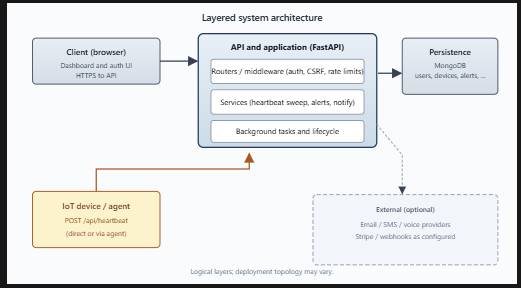
\includegraphics[width=0.92\textwidth]{figures/ICA1_embed_5.png}
  \caption{Figure  System Architecture}
  \label{fig:ica1_5}
\end{figure}

\section{Frontend Design}

The frontend is designed to prioritise clarity and ease of use for non-expert users. A dashboard-centric interface provides a consolidated view of all registered devices, their current availability status, and recent alerts. Visual indicators are used to distinguish between normal operation and abnormal conditions, reducing cognitive load for users.

Core frontend components include:

A login and authentication interface to ensure secure access.

A device management view allowing users to add, edit, or remove registered devices.

A monitoring dashboard presenting real-time status and historical trends.

An alert view highlighting active and resolved incidents.

The frontend design deliberately avoids excessive configuration options, reflecting the requirement for usability and accessibility. Instead, sensible defaults are applied to monitoring thresholds, with limited customisation available for advanced users.

\begin{figure}[htbp]
  \centering
  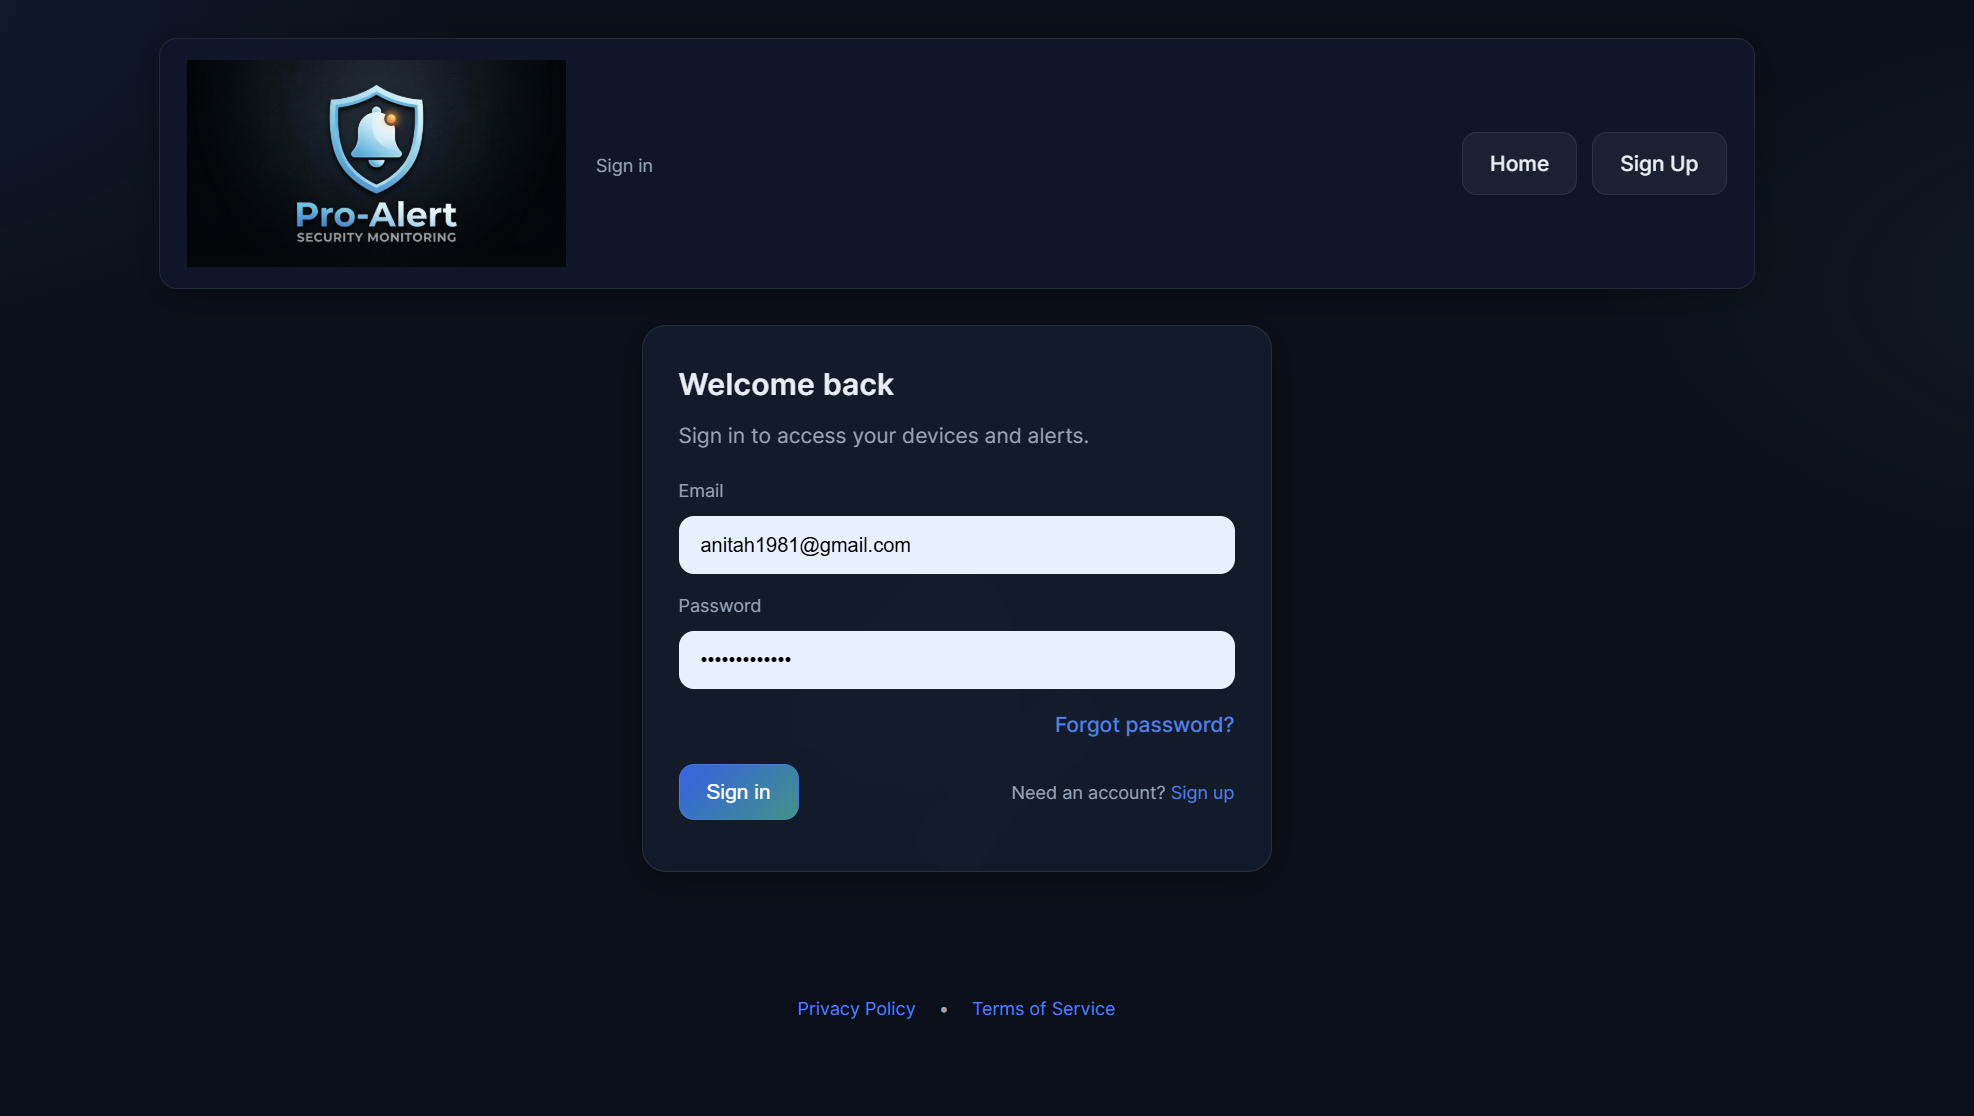
\includegraphics[width=0.92\textwidth]{figures/ICA1_embed_6.png}
  \caption{Figure  Login and Authentication Interface}
  \label{fig:ica1_6}
\end{figure}

\begin{figure}[htbp]
  \centering
  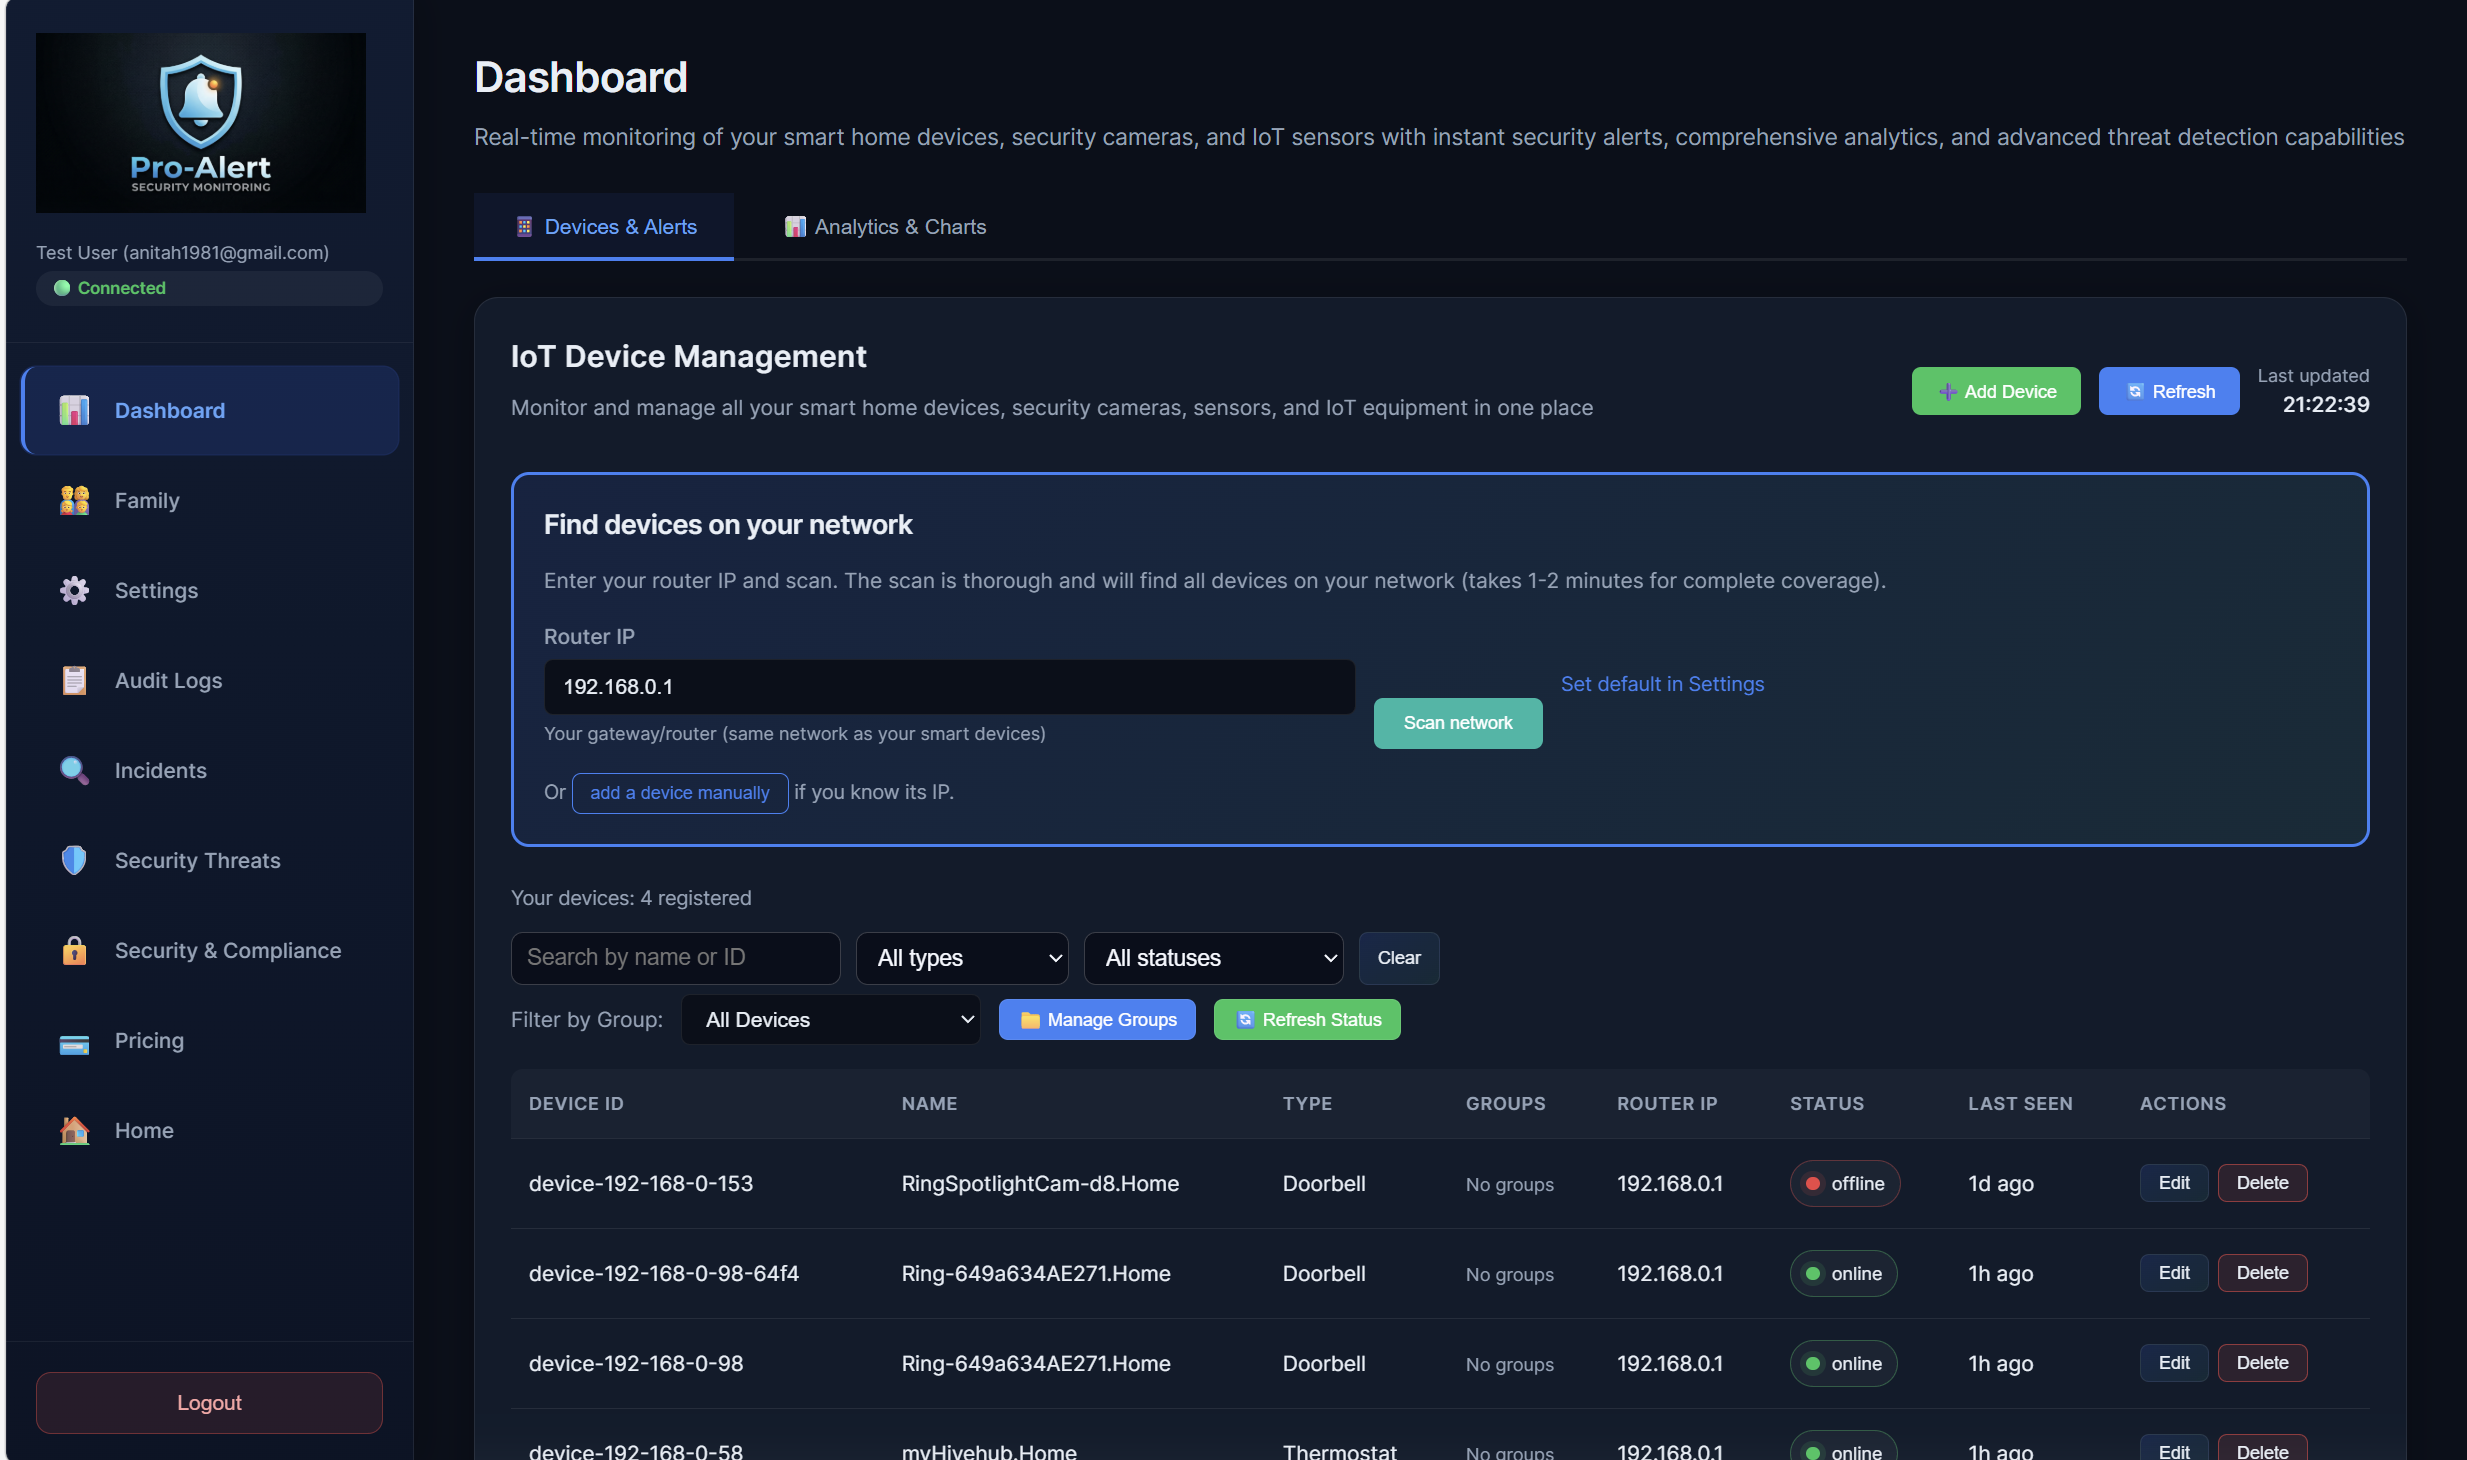
\includegraphics[width=0.92\textwidth]{figures/ICA1_embed_7.png}
  \caption{Figure  Dashboard}
  \label{fig:ica1_7}
\end{figure}

\begin{figure}[htbp]
  \centering
  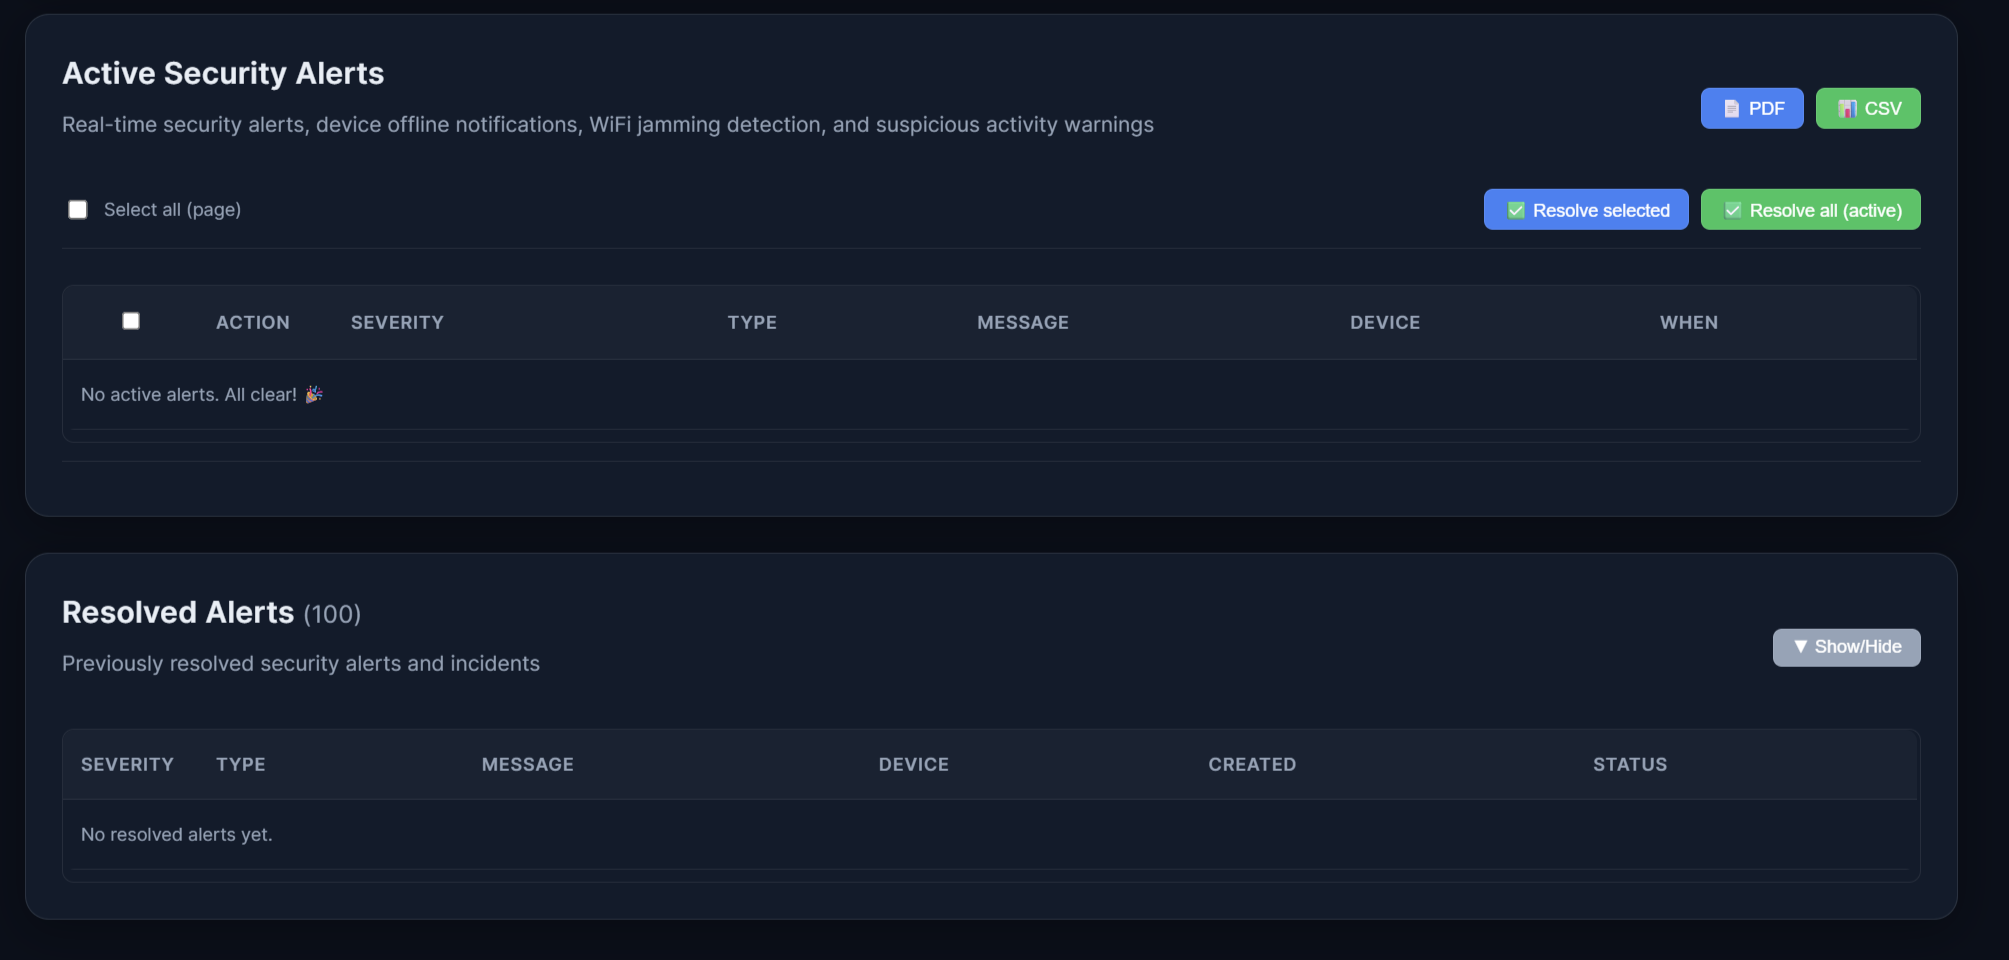
\includegraphics[width=0.92\textwidth]{figures/ICA1_embed_8.png}
  \caption{Figure  Active and Resolved Alerts}
  \label{fig:ica1_8}
\end{figure}

\section{Backend Design}

The backend serves as the central control point for system logic and security enforcement. It exposes a set of API endpoints that facilitate communication between the frontend and backend services. Authentication and authorisation mechanisms ensure that users can only access their own device data.

Key backend responsibilities include:

Managing user accounts and authentication sessions.

Handling device registration and maintaining unique device identifiers.

Receiving and processing heartbeat signals.

Detecting availability failures and anomalous behaviour.

Generating and dispatching alerts.

The backend is implemented using a modular design approach, with distinct services or modules responsible for specific functionality. This modularity supports maintainability and aligns with the non-functional requirement for future extensibility.

\section{Heartbeat Monitoring Mechanism}

Heartbeat monitoring is a core design feature of the system and underpins availability detection. Each registered device is expected to report its presence at regular intervals, either directly or via an intermediary process. The backend records the timestamp of each received heartbeat and compares it against expected intervals.

If a heartbeat is not received within a predefined tolerance window, the system flags the device as potentially unavailable. This approach enables detection of both accidental disconnections and deliberate interference, such as Wi-Fi jamming (TechHive, 2024). The tolerance window is designed to balance responsiveness with resilience to transient network issues, reducing the likelihood of false positives.

Heartbeat data is logged persistently to support historical analysis and evaluation.

\begin{figure}[htbp]
  \centering
  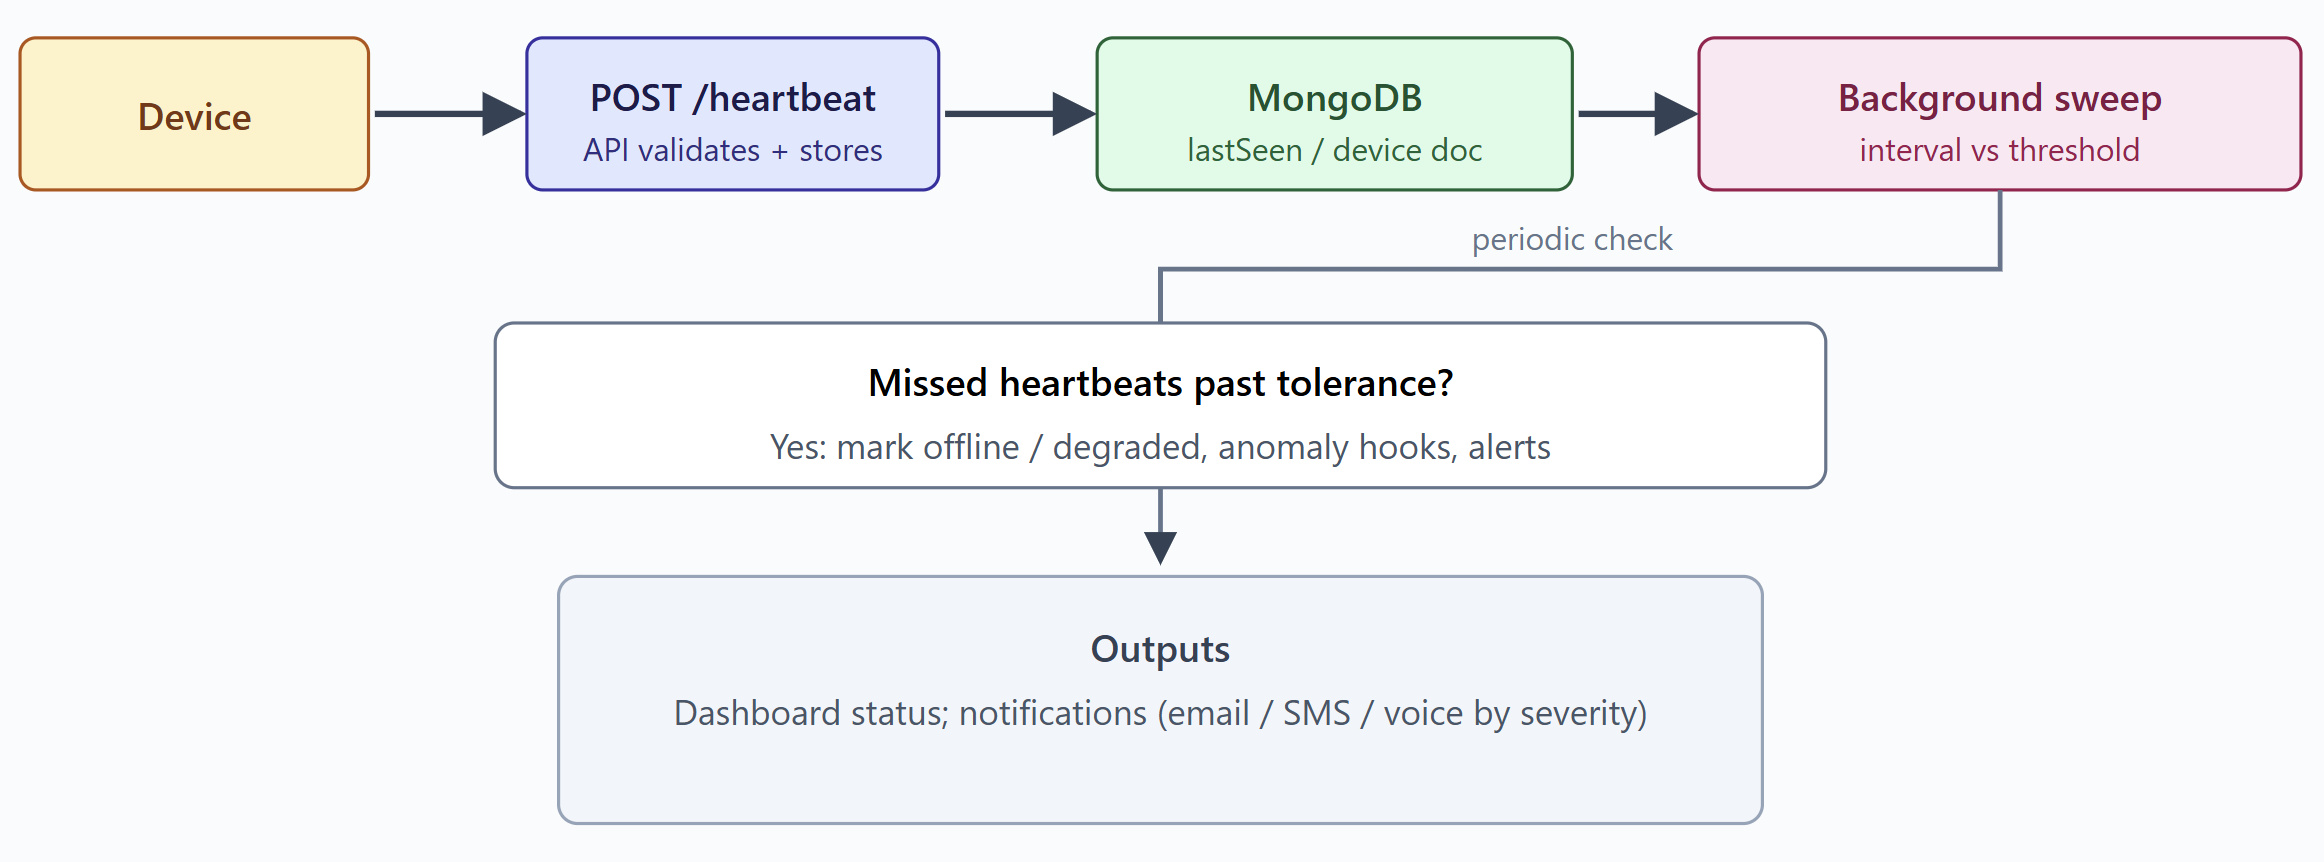
\includegraphics[width=0.92\textwidth]{figures/ICA1_embed_9.png}
  \caption{Figure  Heartbeat Mechanism}
  \label{fig:ica1_9}
\end{figure}

\section{Anomaly Detection Logic}

Anomaly detection within the system is implemented using a behaviour-based approach rather than deep packet inspection. This design choice reflects both resource constraints and privacy considerations, as traditional deep packet inspection is often too heavy and invasive for consumer IoT hardware (Ahmad \& Shah, 2024). The system analyses deviations from expected device behaviour, including irregular heartbeat intervals, repeated disconnections, and sudden status changes.

Multiple indicators are considered when evaluating anomalies, allowing the system to correlate events and improve detection accuracy. For example, a single missed heartbeat may not trigger an alert, whereas repeated missed heartbeats combined with connectivity changes may indicate a more serious issue. This rule- and heuristic-based approach provides transparency and interpretability, enabling users to understand why alerts are generated. It also aligns with the project's emphasis on accessibility and practical deployment.

\section{Alerting and Notification Design}

Alerting is designed to provide timely and actionable information without overwhelming users and risking alert fatigue---a well-documented issue that can lead to users ignoring critical security warnings (Hassan et al., 2020). When availability failures or anomalies are detected, alerts are generated and displayed prominently within the dashboard.

Alerts include contextual information such as device identity, time of occurrence, and the nature of the detected issue. Where feasible, alerts may also be delivered through supplementary notification channels to ensure visibility even when users are not actively monitoring the dashboard. The system supports alert acknowledgement and resolution tracking, enabling users to distinguish between active issues and historical events.

\section{Data Storage and Management}

Persistent storage is used to retain user accounts, device metadata, heartbeat records, and alert logs. Data models are designed to support efficient querying and historical analysis while adhering to data minimisation principles (ICO, 2024). Sensitive information is stored securely, and access controls are enforced at the application level.

Historical data supports both user-facing features, such as trend visualisation, and evaluation activities described in later chapters. Data retention policies are designed to balance analytical value with privacy considerations.

\begin{figure}[htbp]
  \centering
  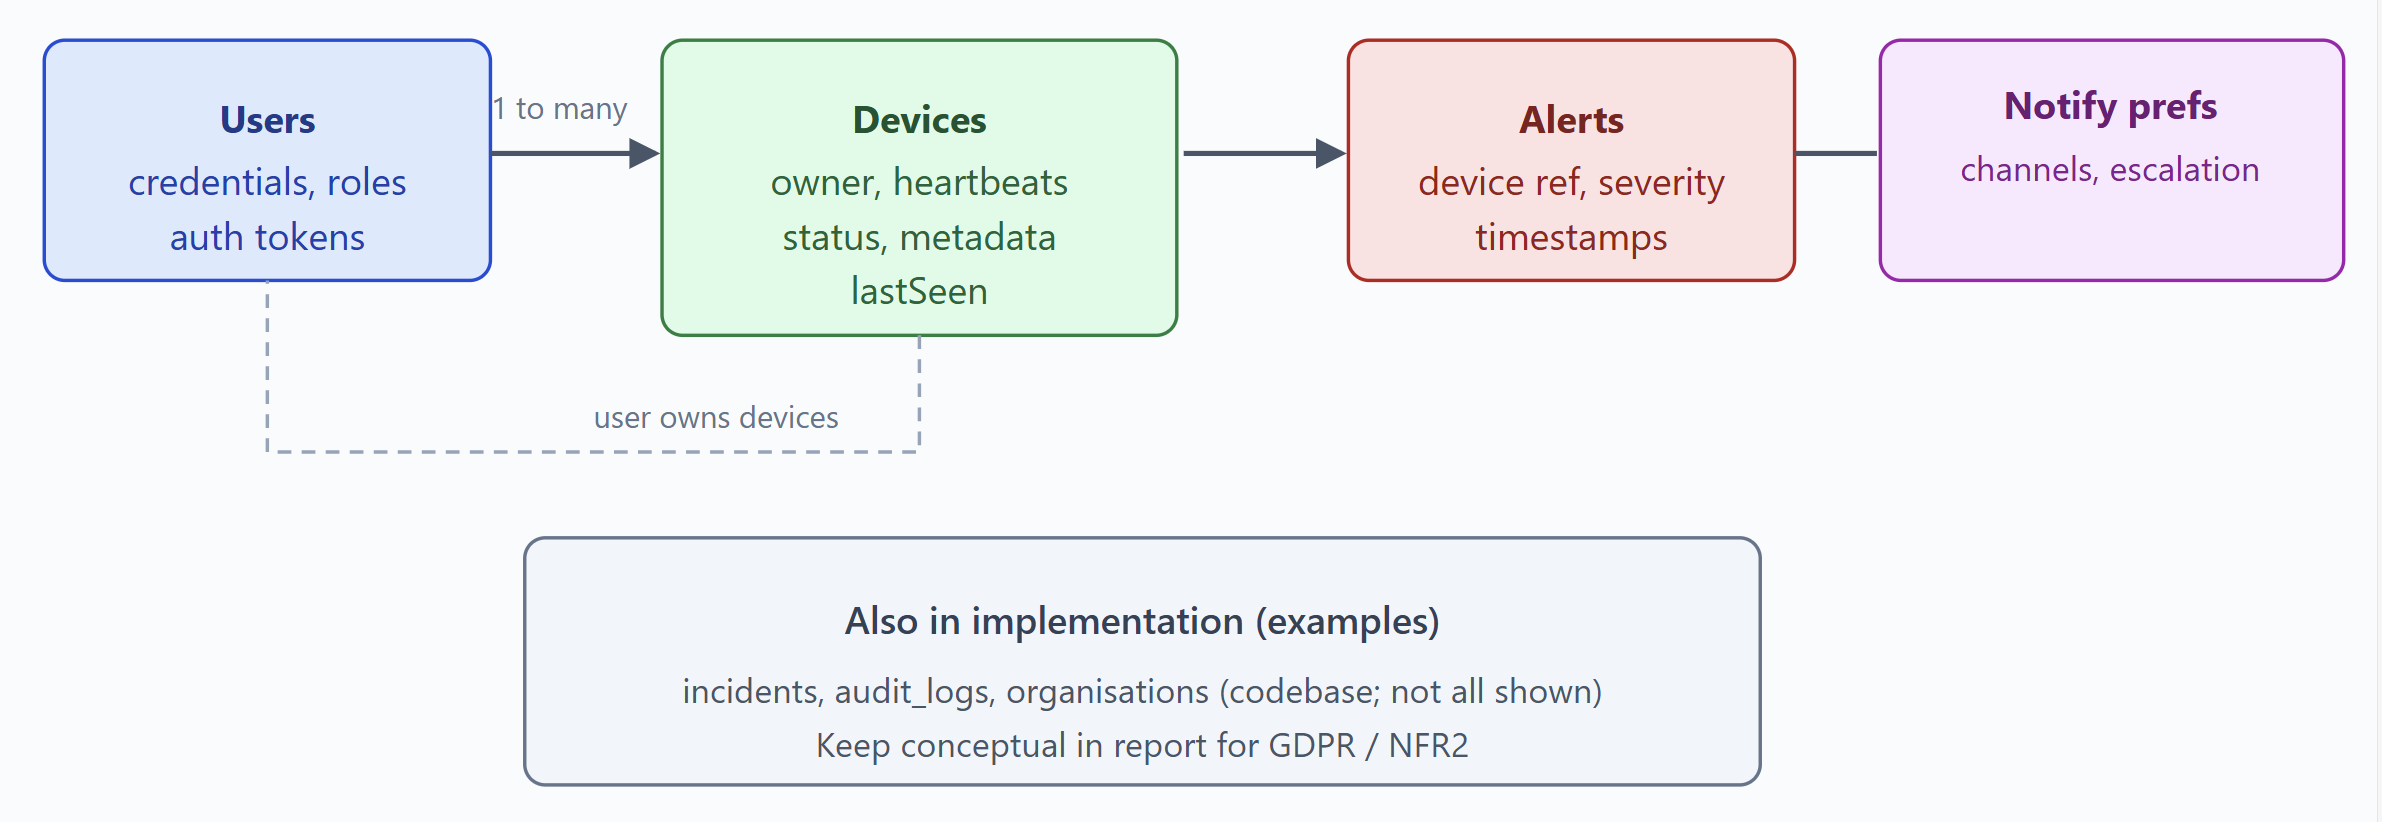
\includegraphics[width=0.92\textwidth]{figures/ICA1_embed_10.png}
  \caption{Figure  Data Storage}
  \label{fig:ica1_10}
\end{figure}

\section{Design Justification and Trade-offs}

Several design trade-offs were made to align the system with project constraints and objectives. The decision to avoid deep packet inspection reduces detection granularity but improves deployability and privacy compliance. Similarly, the use of heuristic-based anomaly detection prioritises transparency and simplicity over advanced machine learning techniques.

These trade-offs are justified by the target deployment context. For home and SMB users, timely awareness of availability and abnormal behaviour provides significant security value without the complexity of enterprise-grade solutions.

\section{Summary}

This chapter has detailed the system design and architectural decisions underpinning the proposed IoT security monitoring application. By mapping requirements to concrete design elements, the chapter demonstrates a structured and intentional approach to system development.

\chapter{Implementation}

\section{Introduction}

This chapter details the implementation of the IoT security monitoring application and explains how the system design outlined in Chapter 9 was translated into a functional software artefact. The implementation focuses on delivering security-driven availability monitoring and anomaly detection while adhering to the functional and non-functional requirements defined in Chapter 8. Particular emphasis is placed on modularity, security, and maintainability to ensure the system is suitable for deployment within home and small-to-medium business (SMB) environments.

\section{Technology Stack and Justification}

The backend of the system was implemented using the FastAPI framework, selected for its high performance, asynchronous processing capabilities, and strong integration with Python type hinting and data validation. FastAPI is particularly well suited to API-driven systems that must handle frequent, lightweight requests, such as IoT heartbeat submissions, while maintaining responsiveness for concurrent users (Hassan et al., 2020).

MongoDB was selected as the primary data store and accessed asynchronously using the Motor driver. This choice supports flexible schema design, which is appropriate for heterogeneous IoT device metadata, while also enabling horizontal scalability. Environment variables are used extensively to manage configuration, allowing sensitive credentials and deployment-specific parameters to be separated from the source code.

The frontend is delivered as a lightweight web-based interface served alongside the API, enabling users to access dashboards, device management views, and alert information without requiring additional client-side installations.

\section{Backend Application Structure}

The backend application follows a modular architecture, separating functionality into clearly defined components, including routing, services, data models, middleware, and database access. This separation of concerns improves readability, maintainability, and extensibility.

Application lifecycle management is handled using FastAPI's lifespan mechanism. During application startup, the system establishes a connection to the MongoDB database, initialises required indexes, and launches background monitoring tasks. On shutdown, database connections are closed gracefully to ensure resource integrity. This structured lifecycle management supports reliability and aligns with best practices for production-grade services.

Routing is organised by functional domain, including authentication, device management, heartbeat processing, alerts, notifications, analytics, audit logging, and incident handling. This organisation reflects the system's core requirements and simplifies future expansion.

\begin{figure}[htbp]
  \centering
  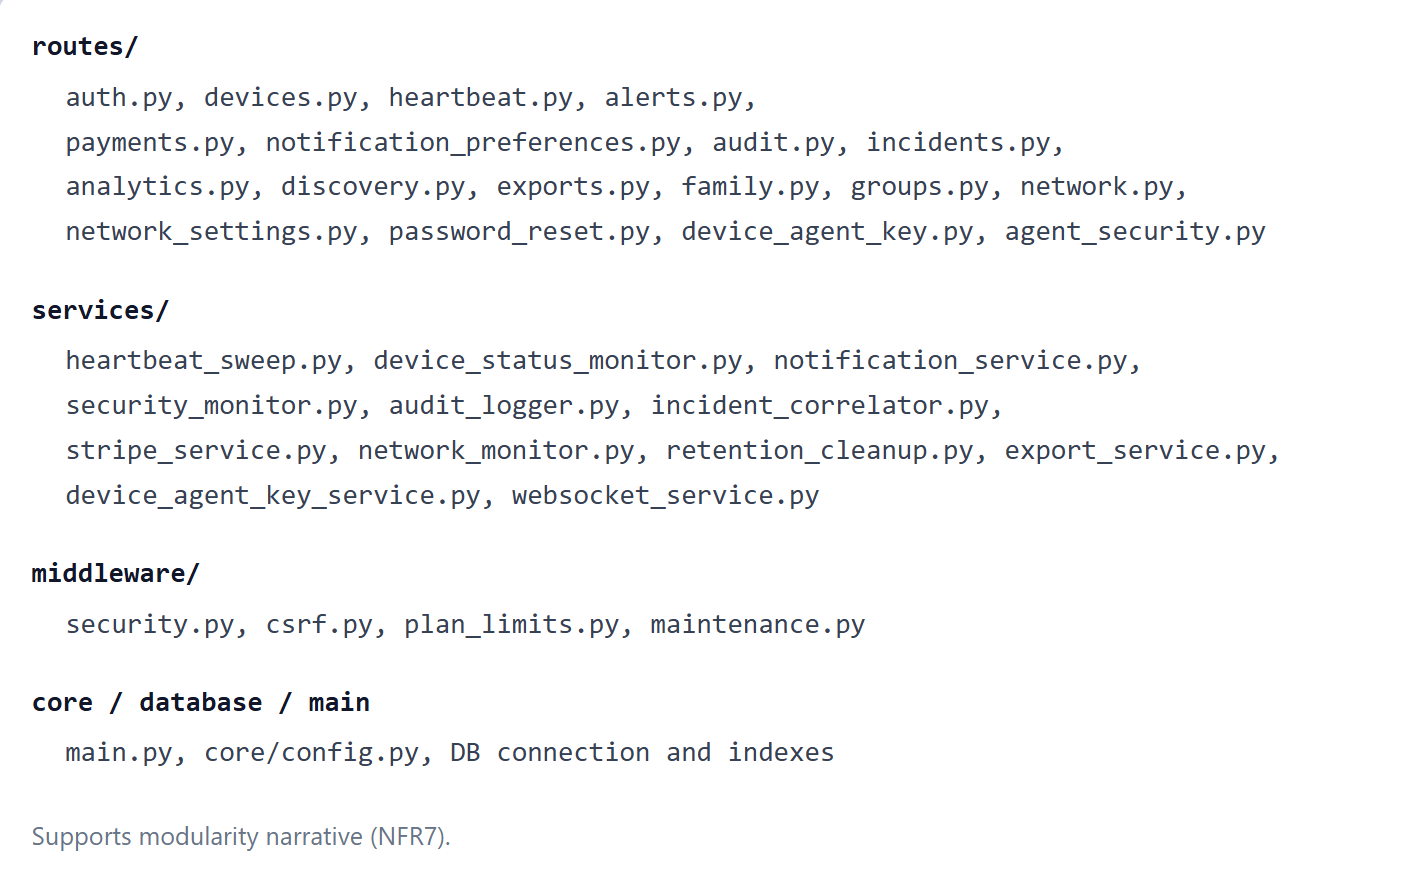
\includegraphics[width=0.92\textwidth]{figures/ICA1_embed_11.png}
  \caption{Figure  Backend Structure}
  \label{fig:ica1_11}
\end{figure}

\section{Data Modelling and Validation}

Data modelling is implemented using Pydantic, providing explicit schema definitions and strong input validation across all core entities. The system defines models for users, devices, alerts, organisations, incidents, notification preferences, and audit logs. Each model enforces constraints such as permitted values, minimum lengths, and required fields.

This approach ensures that invalid or malformed data is rejected at the API boundary, reducing the likelihood of logic errors and improving overall system robustness (OWASP, 2024). Strong typing also improves developer productivity and traceability, as data structures are consistently enforced across the application.

\section{Device Registration and Management}

Device registration is implemented through authenticated API endpoints that allow users to add, update, and remove IoT devices from the monitoring platform. Each device is assigned a logical identifier and associated metadata, including device type, heartbeat interval, network information, and alert preferences.

Device records maintain timestamps for creation, updates, and last-seen activity, enabling both real-time monitoring and historical analysis. Users may adjust configuration parameters such as heartbeat frequency and alert enablement, allowing the system to accommodate devices with different communication characteristics. Device status is updated dynamically based on monitoring outcomes and stored persistently to support trend analysis and evaluation.

\section{Heartbeat Monitoring and Availability Detection}

Heartbeat monitoring constitutes the primary mechanism through which device availability is assessed within the system. Each registered IoT device is expected to submit periodic heartbeat messages to the backend via a dedicated API endpoint. These messages contain the device identifier and may optionally include contextual metadata such as IP address or signal strength. Upon receipt, the backend records the heartbeat timestamp and updates the device's last seen state in persistent storage.

To evaluate ongoing availability, a background monitoring task operates independently of user interaction. This task periodically scans stored heartbeat records and compares the most recent timestamp against a configurable tolerance threshold. If a device fails to report within this window, it is classified as offline or degraded. This approach enables the system to detect both benign failures, such as power loss or network misconfiguration, and more deliberate forms of disruption.

From a security-driven perspective, loss of availability is treated as a potential security incident rather than a purely technical fault. In particular, sustained heartbeat absence may indicate deliberate interference, such as Wi-Fi jamming or network isolation, which can silently disable security-critical devices. Heartbeat thresholds and sweep intervals are configurable via environment settings, allowing the monitoring behaviour to be adapted to different deployment contexts and device characteristics.

\section{Anomaly Detection Logic}

Anomaly detection within the system is implemented using a rule- and heuristic-based approach that focuses on deviations from expected device behaviour. Rather than inspecting network payloads or employing computationally intensive machine learning models, the system analyses observable indicators derived from heartbeat data and device metadata. This design choice prioritises transparency, privacy, and deployability within home and SMB environments (COMPSAC, 2025).

Indicators considered by the system include irregular heartbeat intervals, repeated or prolonged disconnections, sudden changes in IP address, and abnormal signal strength patterns where such data is available. These indicators are evaluated in combination to reduce the likelihood of false positives. For example, a single missed heartbeat may be tolerated, whereas repeated missed heartbeats combined with connectivity changes may trigger a higher-severity alert.

This multi-factor evaluation aligns with the project's emphasis on availability as a security property. By correlating behavioural indicators over time, the system can distinguish between transient network issues and patterns that suggest abnormal or potentially malicious activity. The heuristic-based approach also ensures that alert generation remains interpretable, allowing users to understand why a device has been flagged.

\section{Alerting and Notification Mechanisms}

When availability failures or anomalous behaviour are detected, the system generates alerts that are categorised by type and severity. Alert types include connectivity-related issues, security anomalies, and system-level events, while severity levels range from low to critical. Each alert is stored persistently and associated with the relevant device, supporting both real-time awareness and historical analysis.

Alerts are surfaced to users through the dashboard interface, where they can be reviewed, acknowledged, and resolved. This supports structured incident handling and reduces the risk of unresolved issues being overlooked. In addition to in-application alerts, the system supports multi-channel notification delivery to ensure timely user awareness.

Notification channels include email, SMS, messaging platforms, and automated voice calls. Users can configure notification preferences to control which channels are used for different alert severities. Escalation logic allows higher-severity alerts to trigger more intrusive notification methods, ensuring critical incidents receive appropriate attention while minimising alert fatigue for lower-priority events (NCSC, 2023).

\section{Security Controls and Safeguards}

Security considerations are integrated throughout the implementation to protect both the system and its users. Access to protected resources is enforced through token-based authentication, ensuring that only authorised users can manage devices and view monitoring data. Role-based checks further restrict access to sensitive functionality where applicable.

Input sanitisation and request logging middleware are employed to mitigate common web application threats and support auditability. Rate limiting is implemented to reduce the risk of abuse or denial-of-service attacks, particularly against authentication and monitoring endpoints. Trusted host enforcement and HTTPS redirection are applied in production environments to protect against host header attacks and insecure transport.

API documentation interfaces are disabled by default and made accessible only to authenticated users. This reduces unnecessary information exposure and aligns with the principle of least privilege (OWASP, 2024). Sensitive configuration values, such as database credentials and API keys, are managed exclusively through environment variables rather than being embedded in source code.

\section{Database Management and Performance Considerations}

Database access is managed through a centralised connection layer that initialises and closes connections as part of the application lifecycle. MongoDB is accessed asynchronously using the Motor driver, enabling non-blocking database operations and improved performance under concurrent load.

To support efficient querying, indexes are created on frequently accessed fields, including device identifiers, status values, and timestamp fields such as last seen and alert creation time. These indexes improve responsiveness when listing devices, retrieving alerts, or performing availability sweeps.

Asynchronous database operations allow the system to handle frequent heartbeat submissions and background monitoring tasks without degrading user-facing performance. This design supports scalability as the number of registered devices increases and aligns with the non-functional requirements for performance and reliability.

\section{Implementation Limitations}

Although the implementation delivers the core objectives of the project, several limitations remain. Anomaly detection relies on heuristic rules rather than adaptive or learning-based techniques, which may reduce accuracy in highly dynamic or noisy network environments. Threshold-based approaches also require careful tuning to balance sensitivity against false positives (Ahmad \& Shah, 2024).

Notification delivery depends on third-party services, introducing external dependencies that may affect reliability or incur operational costs in a production setting. Additionally, the system has been developed as a prototype suitable for academic evaluation rather than as a fully hardened commercial product.

Despite these limitations, the modular architecture and configuration-driven design provide a strong foundation for future enhancement, including more advanced detection techniques and improved resilience mechanisms.

\section{Summary}

This chapter has described the implementation of the IoT security monitoring application, focusing on the mechanisms used to detect availability loss, anomalous behaviour, and potential security incidents. The system combines heartbeat-based monitoring, heuristic anomaly detection, and multi-channel alerting to provide meaningful visibility into IoT device status for home and SMB users.

By integrating security controls, performance considerations, and privacy-conscious design choices, the implementation demonstrates a structured and defensible approach to addressing the problem defined earlier in the report.

\chapter{Testing and Evaluation}

\section{Introduction}

This chapter evaluates the IoT security monitoring application by assessing its functional correctness, reliability, and effectiveness in meeting the project objectives. Evaluation is conducted from both an objective perspective, through structured testing of system functionality, and a subjective perspective, through critical reflection on system behaviour, limitations, and overall success.

The testing strategy focuses on validating availability monitoring, anomaly detection, alerting behaviour, and security controls, as these represent the core contributions of the project. Given the academic nature of the artefact, testing is performed using a combination of manual functional testing, simulated failure scenarios, and observational analysis.

\section{Testing Strategy}

A black-box functional testing approach was adopted to evaluate system behaviour from the user's perspective, complemented by targeted white-box observations of backend behaviour through logs and database state. This approach was selected to reflect realistic usage scenarios while remaining appropriate for an undergraduate project context.

Testing was structured around the following key areas:

Device registration and management

Heartbeat submission and availability tracking

Detection of availability failures and anomalous behaviour

Alert generation and notification escalation

Security and access control mechanisms

System robustness under abnormal conditions

Rather than attempting exhaustive testing, the strategy prioritised critical paths that directly support the project's security-driven objectives.

\section{Functional Testing}

Device Registration and Management

Device registration functionality was tested by creating multiple IoT device entries through the authenticated API and dashboard interface. Tests confirmed that devices could be added, updated, and removed successfully, and that each device was uniquely identifiable within the system.

Device metadata, including device type, heartbeat interval, and alert preferences, was stored persistently and retrieved correctly. Invalid inputs, such as missing required fields or unsupported values, were rejected by the system, demonstrating effective input validation.

Outcome: Device management functionality behaved as expected and satisfied the functional requirements for device registration and configuration.

Heartbeat Monitoring and Availability Detection

Heartbeat functionality was tested by submitting periodic heartbeat messages for registered devices and observing changes in availability status. Devices that submitted heartbeats within the expected interval were correctly marked as online, with timestamps updated accordingly.

To simulate availability failures, heartbeat submissions were deliberately halted. After the configured tolerance threshold was exceeded, the system correctly flagged affected devices as offline or degraded. These state changes were recorded persistently and reflected accurately in the dashboard.

Outcome: Heartbeat monitoring reliably detected both normal operation and availability loss, supporting the project's central objective of availability-based security awareness.

Anomaly Detection Behaviour

Anomaly detection was evaluated by simulating abnormal conditions, including repeated missed heartbeats, sudden connectivity changes, and inconsistent reporting patterns. In isolation, minor irregularities did not immediately trigger high-severity alerts. However, when irregularities persisted or occurred in combination, the system generated alerts of increasing severity.

This behaviour demonstrated that the heuristic-based detection logic was capable of distinguishing between transient issues and more concerning patterns indicative of abnormal or potentially malicious activity.

Outcome: The anomaly detection logic functioned as intended, balancing sensitivity with resilience to false positives.

\section{Alerting and Notification Testing}

Alert generation was tested by triggering both availability failures and anomalous behaviour. Alerts were created with appropriate classifications and severity levels and were visible within the dashboard interface. Users were able to acknowledge and resolve alerts, supporting basic incident handling workflows.

Notification delivery was tested across supported channels where configuration was available. Severity-based escalation rules were observed to function correctly, with higher-severity alerts triggering more prominent notification methods. This validation ensures the system can escalate critical threats while actively mitigating alert fatigue for low-level anomalies (Hassan et al., 2020).

Outcome: Alerting and notification mechanisms provided timely and actionable feedback, reinforcing the system's role as a monitoring and awareness tool rather than a passive logging platform.

\section{Security and Access Control Evaluation}

Security controls were evaluated by attempting unauthorised access to protected endpoints and resources. API endpoints requiring authentication were inaccessible without valid credentials, and access to user-specific data was appropriately restricted.

Rate limiting and request validation mechanisms were observed to function as intended, reducing the risk of abuse or accidental overload in alignment with industry-standard API security practices (OWASP, 2024). API documentation interfaces were not publicly accessible and required authentication, limiting information exposure.

Outcome: The system demonstrated appropriate security controls for its intended scope and deployment context.

\section{Performance and Reliability Considerations}

Performance was evaluated qualitatively by observing system behaviour under repeated heartbeat submissions and concurrent user interactions. The asynchronous design enabled the system to process monitoring events without noticeable degradation in responsiveness.

Background monitoring tasks operated independently of user-facing requests, supporting continuous availability evaluation without blocking normal operation. Database indexing further contributed to acceptable query performance when retrieving device and alert data.

Outcome: While formal load testing was beyond the scope of the project, observed performance was consistent with the system's design goals and non-functional requirements.

\begin{figure}[htbp]
  \centering
  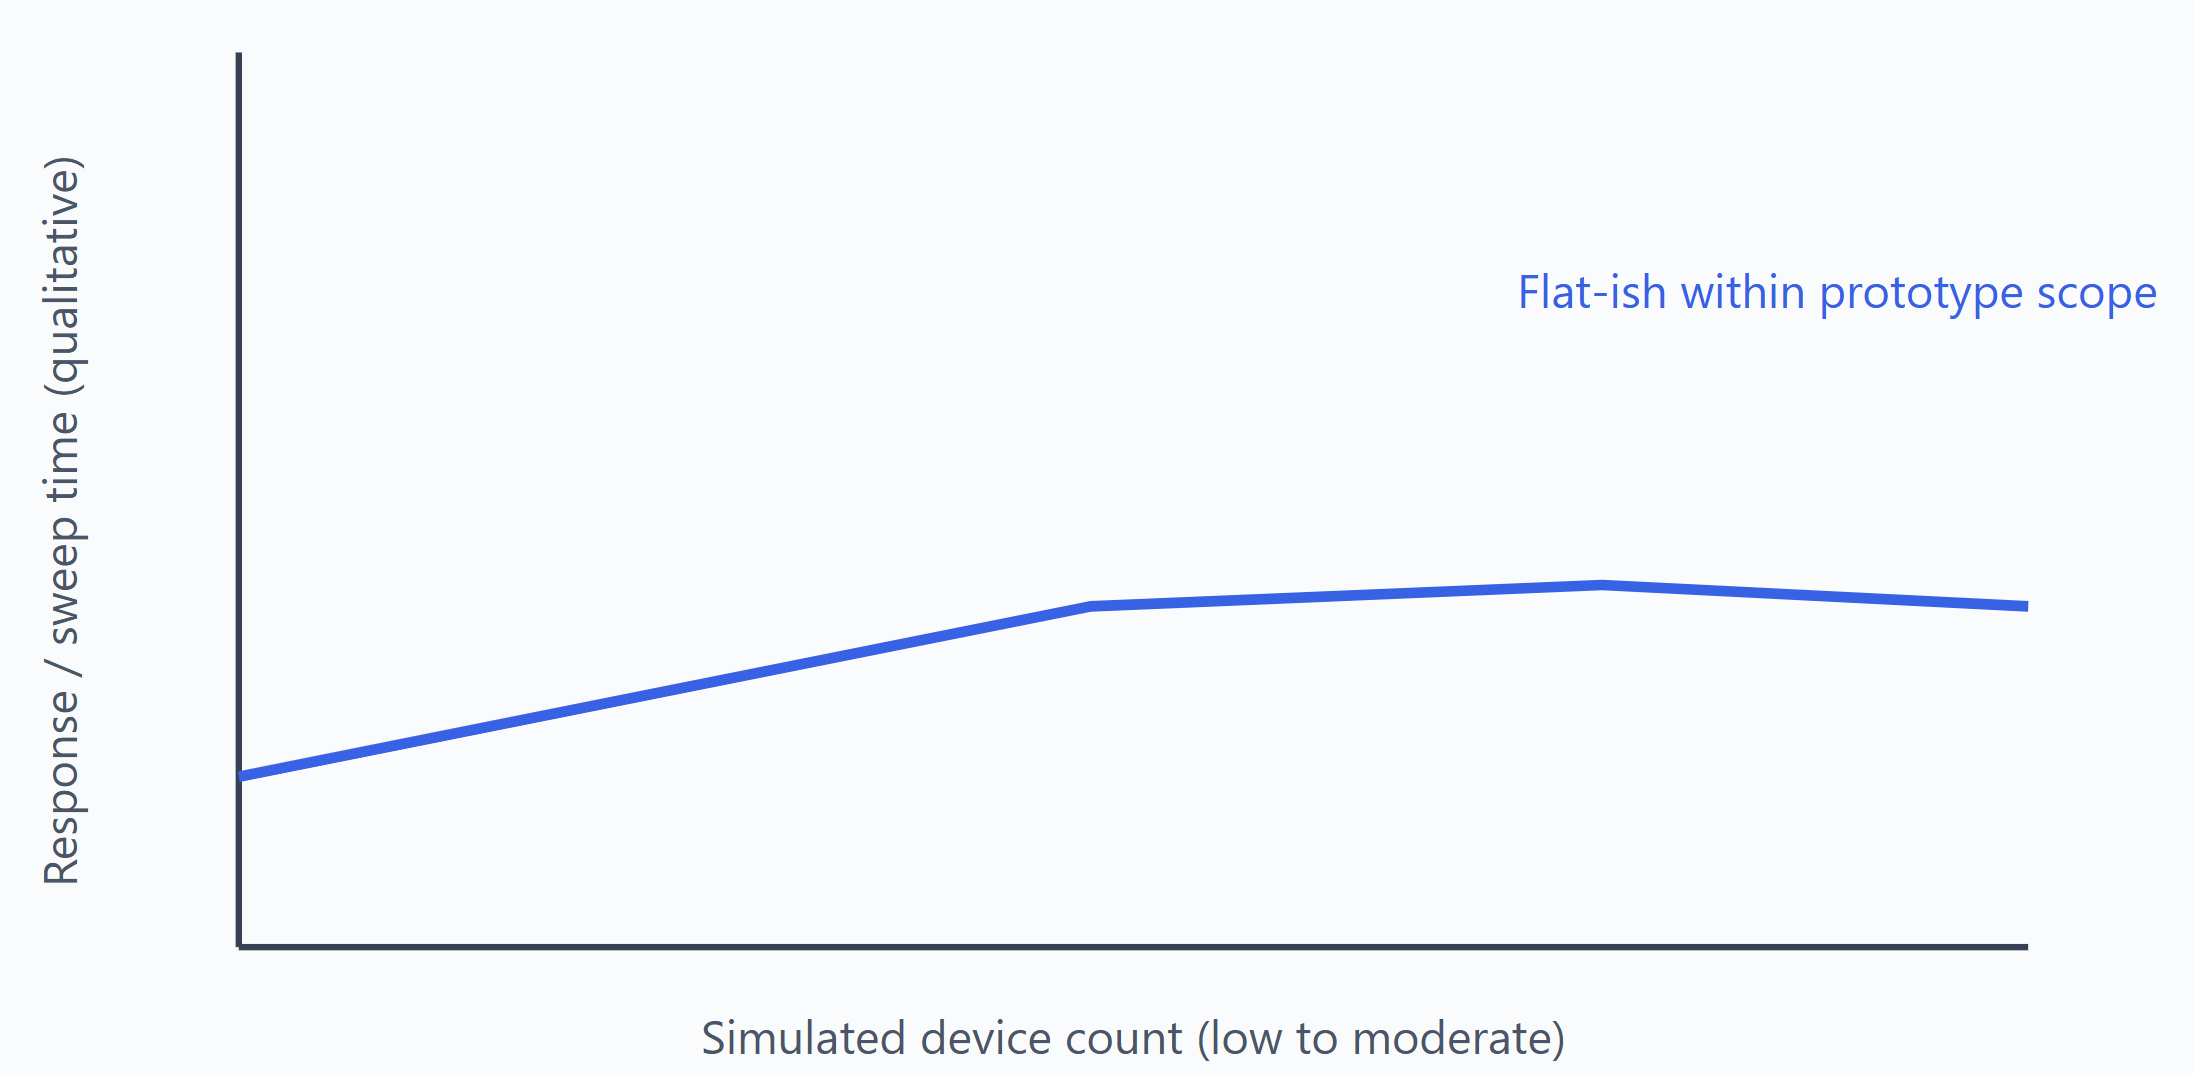
\includegraphics[width=0.92\textwidth]{figures/ICA1_embed_12.png}
  \caption{Figure  Qualitative Performance}
  \label{fig:ica1_12}
\end{figure}

\section{Limitations of Testing}

Several limitations affect the evaluation. Testing was conducted in a controlled environment with a limited number of simulated devices, which may not fully represent large-scale or highly dynamic deployments. Additionally, anomaly detection behaviour was evaluated qualitatively rather than through statistical analysis, reflecting the heuristic nature of the implementation when compared to machine-learning models (Ahmad \& Shah, 2024).

Notification testing depended on external services, which may behave differently under production constraints. These limitations are acknowledged and reflect the scope and constraints of an undergraduate project.

\section{Overall Evaluation of Project Success}

From an objective standpoint, the system successfully meets its core aims. It provides real-time visibility into IoT device availability, detects anomalous behaviour, and delivers timely alerts through configurable notification channels. The implementation demonstrates a coherent integration of security, availability monitoring, and usability considerations.

From a subjective perspective, the project represents a meaningful and practical response to a real-world problem. The focus on availability as a security concern, combined with lightweight monitoring techniques, results in a system that is accessible to non-expert users while still providing tangible security value.

\section{Summary}

This chapter has evaluated the IoT security monitoring application through structured testing and critical analysis. The results demonstrate that the system performs reliably within its intended scope and effectively addresses the problem identified earlier in the report. Identified limitations provide a basis for future improvement, which is explored in the following chapter.

\chapter{Critical Reflection and Discussion}

\section{Introduction}

This chapter provides a critical reflection on the development of the IoT security monitoring application. It evaluates the project from both a technical and personal perspective, considering what was achieved, the challenges encountered, and the effectiveness of the processes used. The discussion also reflects on how design decisions influenced the final artefact and identifies lessons learned throughout the project lifecycle.

\section{Achievement of Project Objectives}

The primary aim of the project was to design and implement a security-driven IoT monitoring application capable of detecting availability loss and anomalous behaviour in home and small-to-medium business (SMB) environments. This aim was largely achieved through the successful implementation of device registration, heartbeat monitoring, anomaly detection, and multi-channel alerting.

The system provides continuous visibility into device availability and responds appropriately to abnormal conditions, aligning with the objectives defined in section 5.3. By focusing on availability as a security concern, the project delivers practical security value without relying on intrusive or resource-intensive monitoring techniques. The modular architecture and configurable design further support the project's original scope and constraints.

\section{Design and Implementation Decisions}

Several key design decisions significantly shaped the final system. The choice to use a heartbeat-based monitoring approach enabled lightweight availability detection while preserving user privacy. This decision avoided deep packet inspection and reduced ethical and legal concerns associated with monitoring network traffic content.

Similarly, the decision to employ heuristic-based anomaly detection rather than machine learning simplified implementation and improved transparency. While this approach limits detection sophistication, it ensures that alert behaviour is understandable to non-expert users and appropriate for the intended deployment context (ENISA, 2023).

The use of FastAPI and an asynchronous database driver supported scalability and responsiveness, particularly for frequent monitoring events. These choices reflect an intentional balance between technical ambition and practical feasibility within the constraints of an undergraduate project.

\section{Challenges Encountered}

The project presented several challenges during development. One significant challenge was managing system complexity while maintaining usability. As features such as alert escalation, notification preferences, and incident handling were added, care was required to prevent the system from becoming overly complex for its target audience---a common pitfall that often leads to security tools being abandoned by non-expert users (Bugcrowd, 2026).

Another challenge involved balancing detection sensitivity with false positives. Availability monitoring and anomaly detection inherently involve threshold-based decisions, and selecting appropriate values required iterative testing and refinement to mitigate the industry-wide challenge of alert fatigue (ResearchGate, 2025). Additionally, reliance on third-party notification services introduced external dependencies that required careful configuration and error handling.

Time constraints also influenced development priorities, requiring a focus on core functionality rather than advanced optimisation or large-scale testing.

\section{Evaluation of Development Process}

The development process followed an incremental and iterative approach, allowing functionality to be implemented and validated progressively. This approach proved effective in managing complexity and identifying issues early in development.

Requirements analysis and design documentation provided a clear reference point throughout implementation, reducing the risk of scope creep and supporting coherent system development. However, more formalised testing earlier in the process could have further improved reliability and reduced rework during later stages.

Overall, the chosen development methodology was appropriate for the project scope and contributed positively to the quality of the final artefact.

\section{Personal Reflection and Skills Development}

From a personal perspective, the project facilitated significant skill development across multiple areas. Technical skills were strengthened through hands-on experience with backend development, asynchronous programming, database design, and security middleware. The project also enhanced understanding of IoT security challenges and the practical trade-offs involved in real-world system design.

Beyond technical skills, the project improved problem-solving, planning, and critical evaluation abilities. Managing a complex system independently required effective time management and decision-making, reinforcing skills relevant to professional software development and cybersecurity roles.

\section{Summary}

This chapter has critically reflected on the project's outcomes, processes, and challenges. The discussion demonstrates that the project achieved its core objectives while operating within defined constraints. Identified limitations and lessons learned provide valuable insight and inform potential future enhancements, which are explored in the following chapter.

\chapter{Future Work and Enhancements}

\section{Introduction}

While the implemented system meets its primary objectives, there are numerous opportunities for future development. This chapter outlines potential enhancements that could improve detection accuracy, scalability, and practical applicability, particularly in production or enterprise-adjacent contexts.

\section{Advanced Anomaly Detection Techniques}

One significant area for future work involves enhancing anomaly detection through adaptive or learning-based techniques. Machine learning models could be introduced to learn baseline device behaviour over time and identify more subtle deviations. Such techniques may reduce false positives and improve detection accuracy in dynamic environments (Ahmad \& Shah, 2024).

However, adopting these approaches would require additional data, training infrastructure, and careful consideration of model interpretability and bias, particularly in safety-critical contexts.

\section{Improved Availability and Resilience Detection}

Future enhancements could incorporate additional indicators to improve availability assessment, such as network latency measurements, packet loss estimation, or correlation across multiple devices. Combining these indicators could improve detection of coordinated attacks, including large-scale jamming or network disruption, which are increasingly targeting wireless IoT layers (Future Internet, 2026).

Redundant monitoring mechanisms and failover alert channels could further improve system resilience, ensuring notifications are delivered even when primary communication paths are unavailable.

\section{Scalability and Performance Enhancements}

To support larger deployments, future versions of the system could integrate message queues or event-streaming platforms to decouple heartbeat ingestion from processing. This would improve scalability and enable more sophisticated analysis pipelines.

Additional performance optimisation could include caching frequently accessed data and implementing horizontal scaling across multiple backend instances.

\section{User Experience and Visualisation Improvements}

Enhancements to the user interface could improve usability and situational awareness. Potential improvements include richer data visualisation, historical trend analysis, and interactive incident timelines. Providing clearer explanations of alert causes and recommended actions could further support non-expert users, reducing confusion during security events (NCSC, 2023).

Mobile application support could also be introduced to improve accessibility and responsiveness to critical alerts.

\section{Integration and Commercial Considerations}

Future work could explore integration with existing smart home platforms, routers, or enterprise monitoring tools. Such integrations would enhance interoperability and reduce deployment friction.

From a commercial perspective, tiered service models, enhanced reporting, and compliance-focused features could be developed to support monetisation and adoption within SMB environments, addressing the gap between consumer products and full-scale enterprise solutions (SumatoSoft, 2025).

\section{Summary}

This chapter has outlined potential avenues for future development that build on the existing system. These enhancements address identified limitations and highlight opportunities to extend the platform's functionality, performance, and applicability. Together, they demonstrate that the project provides a strong foundation for continued development beyond its academic scope.

\chapter{Conclusion}

This project set out to design and implement a security-driven IoT monitoring application capable of improving visibility, availability awareness, and anomaly detection within home and small-to-medium business (SMB) environments. The motivation for the project arose from the growing prevalence of IoT devices and the corresponding lack of accessible security monitoring solutions for non-enterprise users (Hassan et al., 2020).

The project successfully delivered a functional monitoring platform that provides continuous insight into device availability through heartbeat-based monitoring. By treating availability loss as a security concern, the system addresses a critical but often overlooked weakness in consumer and SMB IoT deployments. The use of heuristic anomaly detection enables the identification of abnormal behaviour without relying on intrusive inspection or resource-intensive techniques, aligning with privacy and usability considerations (ICO, 2024).

A structured development process was followed, incorporating requirements analysis, system design, implementation, and evaluation. Each stage was informed by academic research and justified design decisions, resulting in a coherent and defensible artefact. The modular architecture, asynchronous processing model, and multi-channel alerting mechanisms demonstrate a practical balance between technical robustness and deployment feasibility.

Evaluation of the system showed that it performs reliably within its intended scope, accurately detecting availability failures and generating timely alerts. While limitations exist, particularly in relation to detection sophistication and large-scale testing, these constraints are appropriate given the academic context of the project. Importantly, the system provides a strong foundation for future enhancement, including advanced anomaly detection, scalability improvements, and broader integration opportunities.

In conclusion, the project achieves its primary objectives and delivers meaningful security value for home and SMB IoT users. It demonstrates a sound understanding of IoT security challenges and applies appropriate technical solutions within realistic constraints. The work contributes a practical perspective on availability-focused IoT security monitoring and highlights the potential for continued development beyond the scope of this project.

\chapter{References}

Ahmad, T. and Shah, M., 2024. Lightweight mini-batch federated learning technique for efficient attack detection in IoT systems. Journal of IoT Security / JISEM.

Antonakakis, M., April, T., Bailey, M., Bernhard, M., Bursztein, E., Cochran, J., Durumeric, Z., Halderman, J.A., Invernizzi, L., Kallitsis, M. and Kumar, D., 2017. Understanding the Mirai botnet. In 26th USENIX Security Symposium, pp. 1093-1110.

Bugcrowd, 2026. The Human Attack Surface: A Serious Threat to Cybersecurity. [online] Available at: https://www.bugcrowd.com/blog/the-human-attack-surface-a-serious-threat-to-cybersecurity/

COMPSAC, 2025. A Lightweight Monitoring and Anomaly Detection Framework for IoT Devices. Proceedings of the IEEE Computer Society Signature Conference on Computers, Software and Applications.

ENISA, 2023. Good Practices for IoT and Smart Infrastructures Tool. [online] European Union Agency for Cybersecurity. Available at: https://www.enisa.europa.eu/

Fortinet, 2024. Why Are SMBs Most Vulnerable to Cyberattacks?. [online] Available at: https://www.fortinet.com/uk/resources/cyberglossary/smb-cyberattacks

Future Internet, 2026. Multi-Attribute Physical-Layer Authentication Against Jamming and Battery-Depletion Attacks in LoRaWAN. Future Internet Journal, 18(38).

Hassan, W. H., et al., 2020. Security Requirements for the Internet of Things: A Systematic Approach. National Institutes of Health (PMC).

Information Commissioner's Office (ICO), 2024. Data protection and privacy for smart devices. [online] Available at: https://ico.org.uk/for-organisations/uk-gdpr-guidance-and-resources/

IoT Analytics, 2024. State of IoT---Spring 2024. [online] IoT Analytics GmbH. Available at: https://iot-analytics.com/

Journal of Engineering 360, 2024. Vulnerability of Wi-Fi wireless network to signal interference. [online] Available at: https://journalofengineering360.ajp.edu.pl/article/548861/en

Kaspersky, 2024. Internet of Things security challenges and best practices. Kaspersky Resource Center.

Keyfactor, 2024. IoT Device Security: Risks, Best Practices, and Protection Tips. Keyfactor Education Center.

National Cyber Security Centre (NCSC), 2023. Smart devices in the home: a guide for businesses and individuals. [online] Available at: https://www.ncsc.gov.uk/guidance/smart-devices-in-the-home

OAE Publish, 2023. Anatomy of attacks on IoT systems: review of attacks, impacts and countermeasures. Journal of Surveillance, Security and Safety.

Open Worldwide Application Security Project (OWASP), 2024. OWASP Top 10 API Security Risks. [online] Available at: https://owasp.org/API-Security/

R Discovery, 2025. Self-Adaptive Sensor Fault Detection in IoT Health Monitoring Using Federated Learning and Lightweight Transformers. [online] Available at: https://discovery.researcher.life/article/self-adaptive-sensor-fault-detection-in-iot-health-monitoring-using-federated-learning-and-lightweight-transformers/fee363dd342d3637957e563318e15e0e

ResearchGate (Various Authors), 2025. Anomaly Detection in Real-Time IoT Systems Using Machine Learning. ResearchGate Publications.

ResearchGate, 2025. An IoT-Based Smart Framework for a Human Heartbeat Rate Monitoring and Control System. [online] Available at: https://www.researchgate.net/publication/337275306\_An\_IoT-Based\_Smart\_Framework\_for\_a\_Human\_Heartbeat\_Rate\_Monitoring\_and\_Control\_System

RiskRecon, 2023. Security in the Internet of Things. RiskRecon Security Blog.

Roman, R., Zhou, J. and Lopez, J., 2013. On the features and challenges of security and privacy in distributed internet of things. Computer Networks, 57(10), pp. 2266-2279.

SecuringSam, 2023. ``Hot Patching'' -- Seamlessly Protecting the Routers of Your SMB Customers. [online] Available at: https://securingsam.com/hot-patching-seamlessly-protecting-the-routers-of-your-smb-customers/

Sicari, S., Rizzardi, A., Grieco, L.A. and Coen-Porisini, A., 2015. Security, privacy and trust in Internet of Things: The road ahead. Computer Networks, 76, pp. 146-164.

SumatoSoft, 2025. Enterprise IoT Software Development for Businesses. [online] Available at: https://sumatosoft.com/services/enterprise-iot-development

TechHive, 2024. Wi-Fi jamming attacks are on the rise. How they affect your smart home security. [online] Available at: https://www.techhive.com/article/2321439/wifi-jamming-attacks-smart-home-security.html

Weber, R.H., 2010. Internet of Things -- New security and privacy challenges. Computer Law \& Security Review, 26(1), pp. 23-30.

Zarpelão, B.B., Miani, R.S., Kawakani, C.T. and de Alvarenga, S.C., 2017. A survey of intrusion detection in Internet of Things. Journal of Network and Computer Applications, 84, pp. 25-37.
